\chapter{Results and discussions}\label{ch:results}
In this chapter, the vortex analysis of air flow over a solid cylinder using a constant-current hot wire anemometer is discussed.
The vortex analysis is performed at a distance of $D$, $2~D$ and $4~D$ from the cylinder, where $D$ is the diameter of the cylinder. The analysis is also performed at a distance of $0.5~D$ above the cylinder at all the points mentioned above. The air flow is kept at a pitot tube pressure of $1~Pa$, $2~Pa$, $3~Pa$ and $4~Pa$. The results are discussed in the following sections.

\section{Vortex analysis at distance \texorpdfstring{$x=D$}~~from the cylinder}
In this section, the vortex analysis of the flow is done by keeping the hot wire anemometer at a distance of $D$ from the center of the cylinder. Further, the probe is moved to a height of $0.5~D$ above the center of the cylinder, and the same analysis is performed. 
\subsection{Vortex analysis at the center of the cylinder}


\begin{figure}[h]
    \centering
    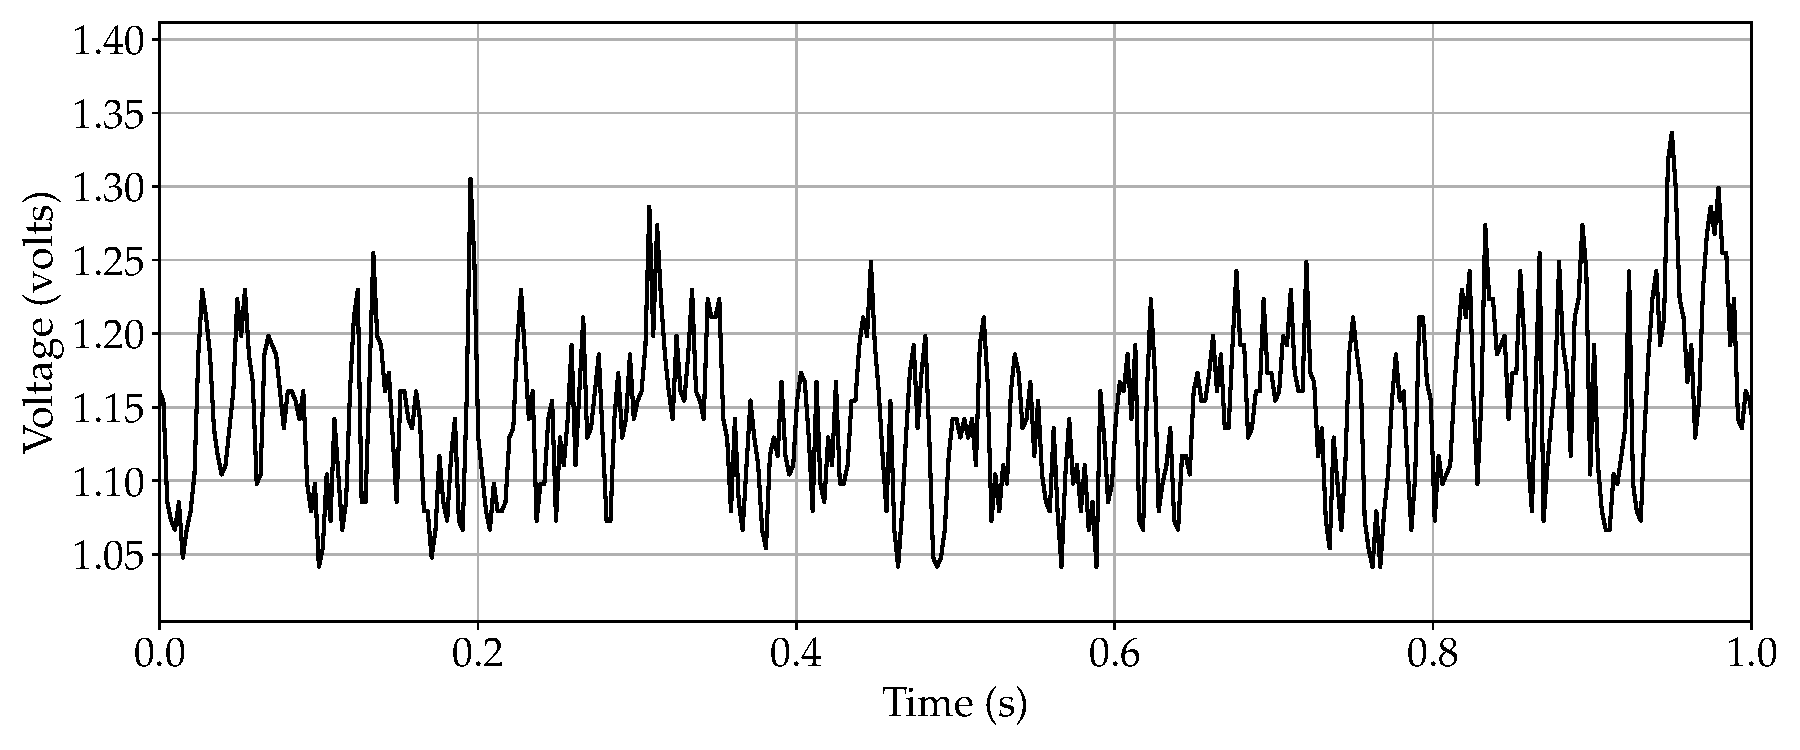
\includegraphics[width=\linewidth]{gfx/voltage_vs_time_for_1Pa_1s.pdf}
    \caption{The variation of voltage with time for a flow having differential pressure of $1~Pa$ for sensor placed at a distance of $D$ from the cylinder}
    \label{fig:vortex_D_1Pa}
\end{figure}

The solid cylinder is kept at a distance of $0.20~m$ from the left end of the test section. The speed of the suction fan is varied from an equivalent differential pressure of $1~Pa$, $2~Pa$, $3~Pa$ and $4~Pa$ using an auto transformer. The output of the hot wire anemometer is recorded in the PC Oscilloscope for a time of $10~s$ for all flow pressures. The voltage variation with time for a flow having differential pressure of $1~Pa$ (between $0~\text{to}~1~s$) is shown in Fig.~\ref{fig:vortex_D_1Pa}.

The interest is to find the velocity fluctuation in the test section due to the presence of a solid cylinder. The voltage output from the oscilloscope is converted to velocity using the calibration equation (see Eq.~(\ref{eq:calib_eqn_hwa})). The corresponding velocity fluctuation with time is shown in Fig.~\ref{fig:vortex_D_1Pa_vel}.

\begin{figure}
    \centering
    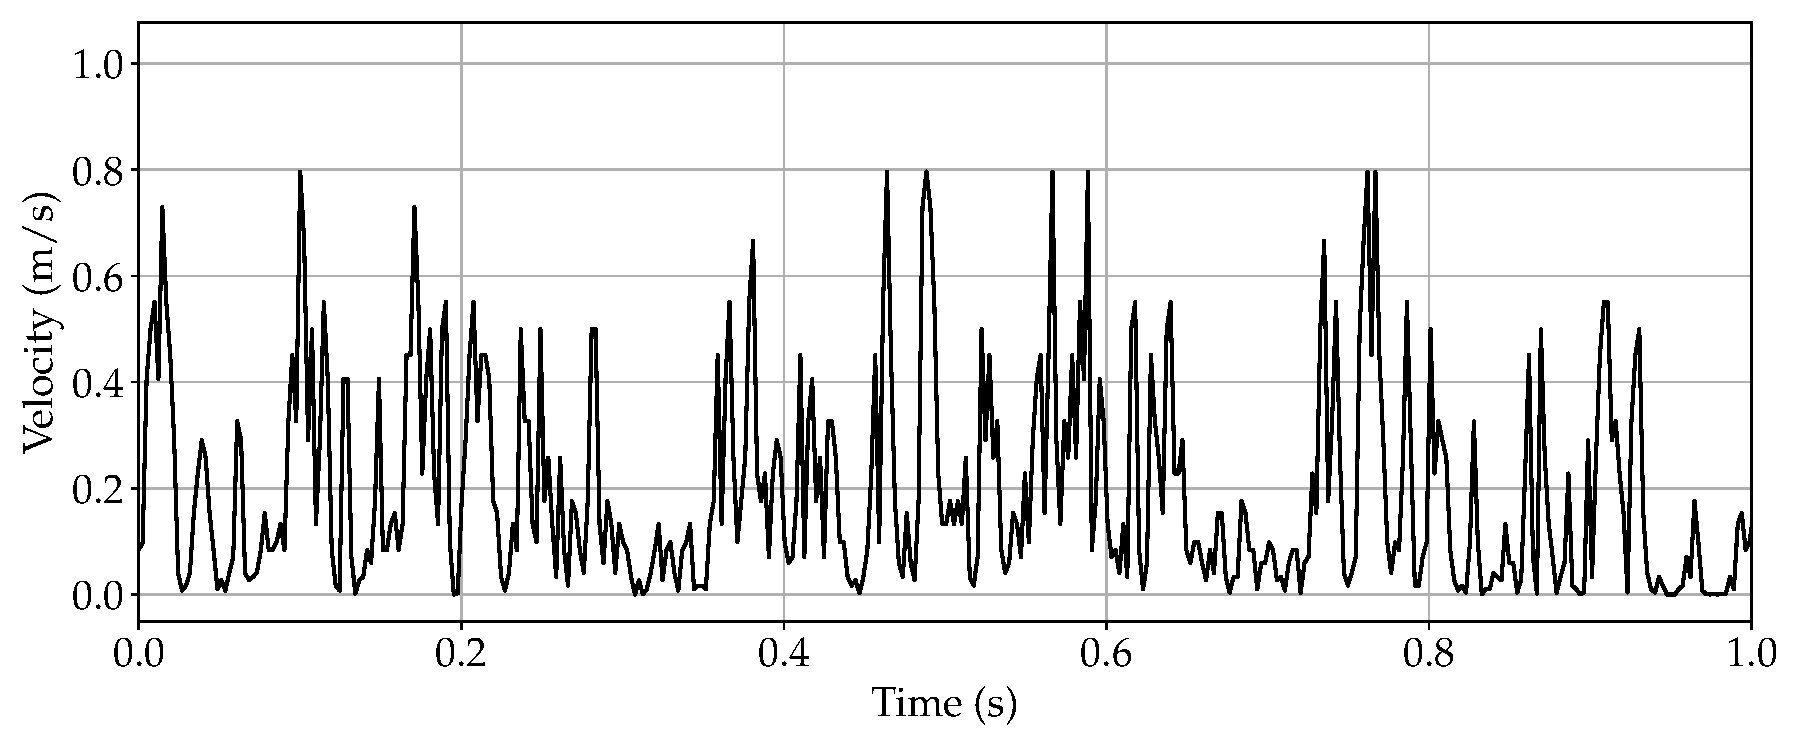
\includegraphics[width=\linewidth]{gfx/velocity_vs_time_for_1Pa_1s.pdf}
    \caption{The variation of velocity with time for a flow having differential pressure of $1~Pa$ for sensor placed at a distance of $D$ from the cylinder}
    \label{fig:vortex_D_1Pa_vel}
\end{figure}
The fluctuation in flow velocity is due to the occurrence of vortices when the flow is obstructed by the solid cylinder. Here, since the velocity varies with time, it can be assumed to be a function of time. That is,
\begin{equation}
    v = v(t).
\end{equation}
Further, the frequency of the vortex can be found by transforming the velocity from temporal domain ($t$) to frequency domain ($\omega$) using the Fourier transform pairs given by

\begin{equation}\label{eq:forward fourier}
        \Hat{V}(\omega) = \frac{1}{2\pi}\int^{\infty}_{-\infty}v(t)e^{-i\omega t}dt
\end{equation}
\begin{equation}\label{eq:backward fourier}
        v(t) = \int^{\infty}_{-\infty}\Hat{V}(\omega)\mathbf{e}^{i\omega t}d\omega
\end{equation}
where $\Hat{V}$ is the transformed velocity and $\omega$ is the frequency in $rad/s$ ($=2\pi f$, f - frequency in $Hz$). The velocity variation is transformed using Eq.~\ref{eq:forward fourier} and resulting frequency variation of velocity spectral density for flow having differential pressure of $1~Pa$ (scaled to 0~$Hz$ to $100~Hz$) is shown in Fig.~\ref{fig:vel_freq_1Pa}.
\begin{figure}
    \centering
    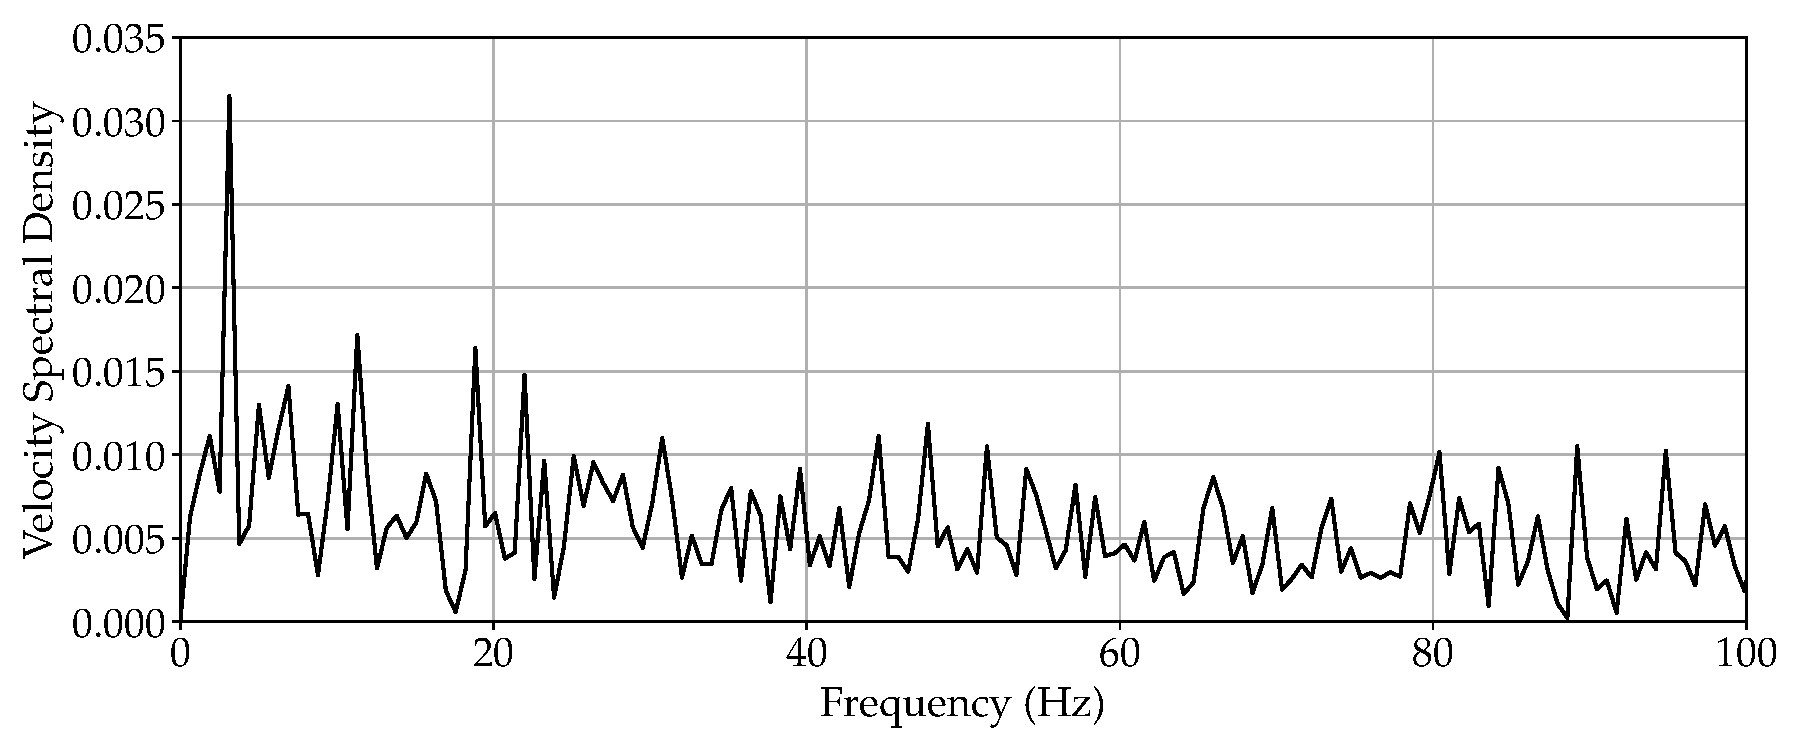
\includegraphics[width=\linewidth]{gfx/FFT_vel_1Pa.pdf}
    \caption{Frequency spectrum of velocity.}
    \label{fig:vel_freq_1Pa}
\end{figure}
In this figure, it can be seen that the velocity spectrum peaks at many frequencies. The maximum peak occurs at a frequency of about $3.14~Hz$, which corresponds to the frequency of the vortex. Similar frequency peaks are also found in other flow pressures of $2~Pa$, $3~Pa$ and $4~Pa$. Eq.~(\ref{eq:press_vel equation}) can be used to find the velocity corresponding to the flow pressure. The Reynolds number for the flow can be calculated using
\begin{equation}\label{eq:reynolds number}
    Re = \frac{\rho U D}{\mu},
\end{equation}
where $\rho$ is the density of air (1.17~$kg/m^3$), $U$ is the flow velocity in $m/s$, $D$ is the diameter of the solid cylinder ($0.033~m$) and $\mu$ is the dynamic viscosity of air ($1.87 \times 10^{-5}~kg/m\cdot s$). A comparison of velocity spectral density with frequency for all flow velocities (written in terms of Reynolds number) is shown in Fig.~\ref{fig:surface_x_D_y_0}.
\begin{figure}
    \centering
    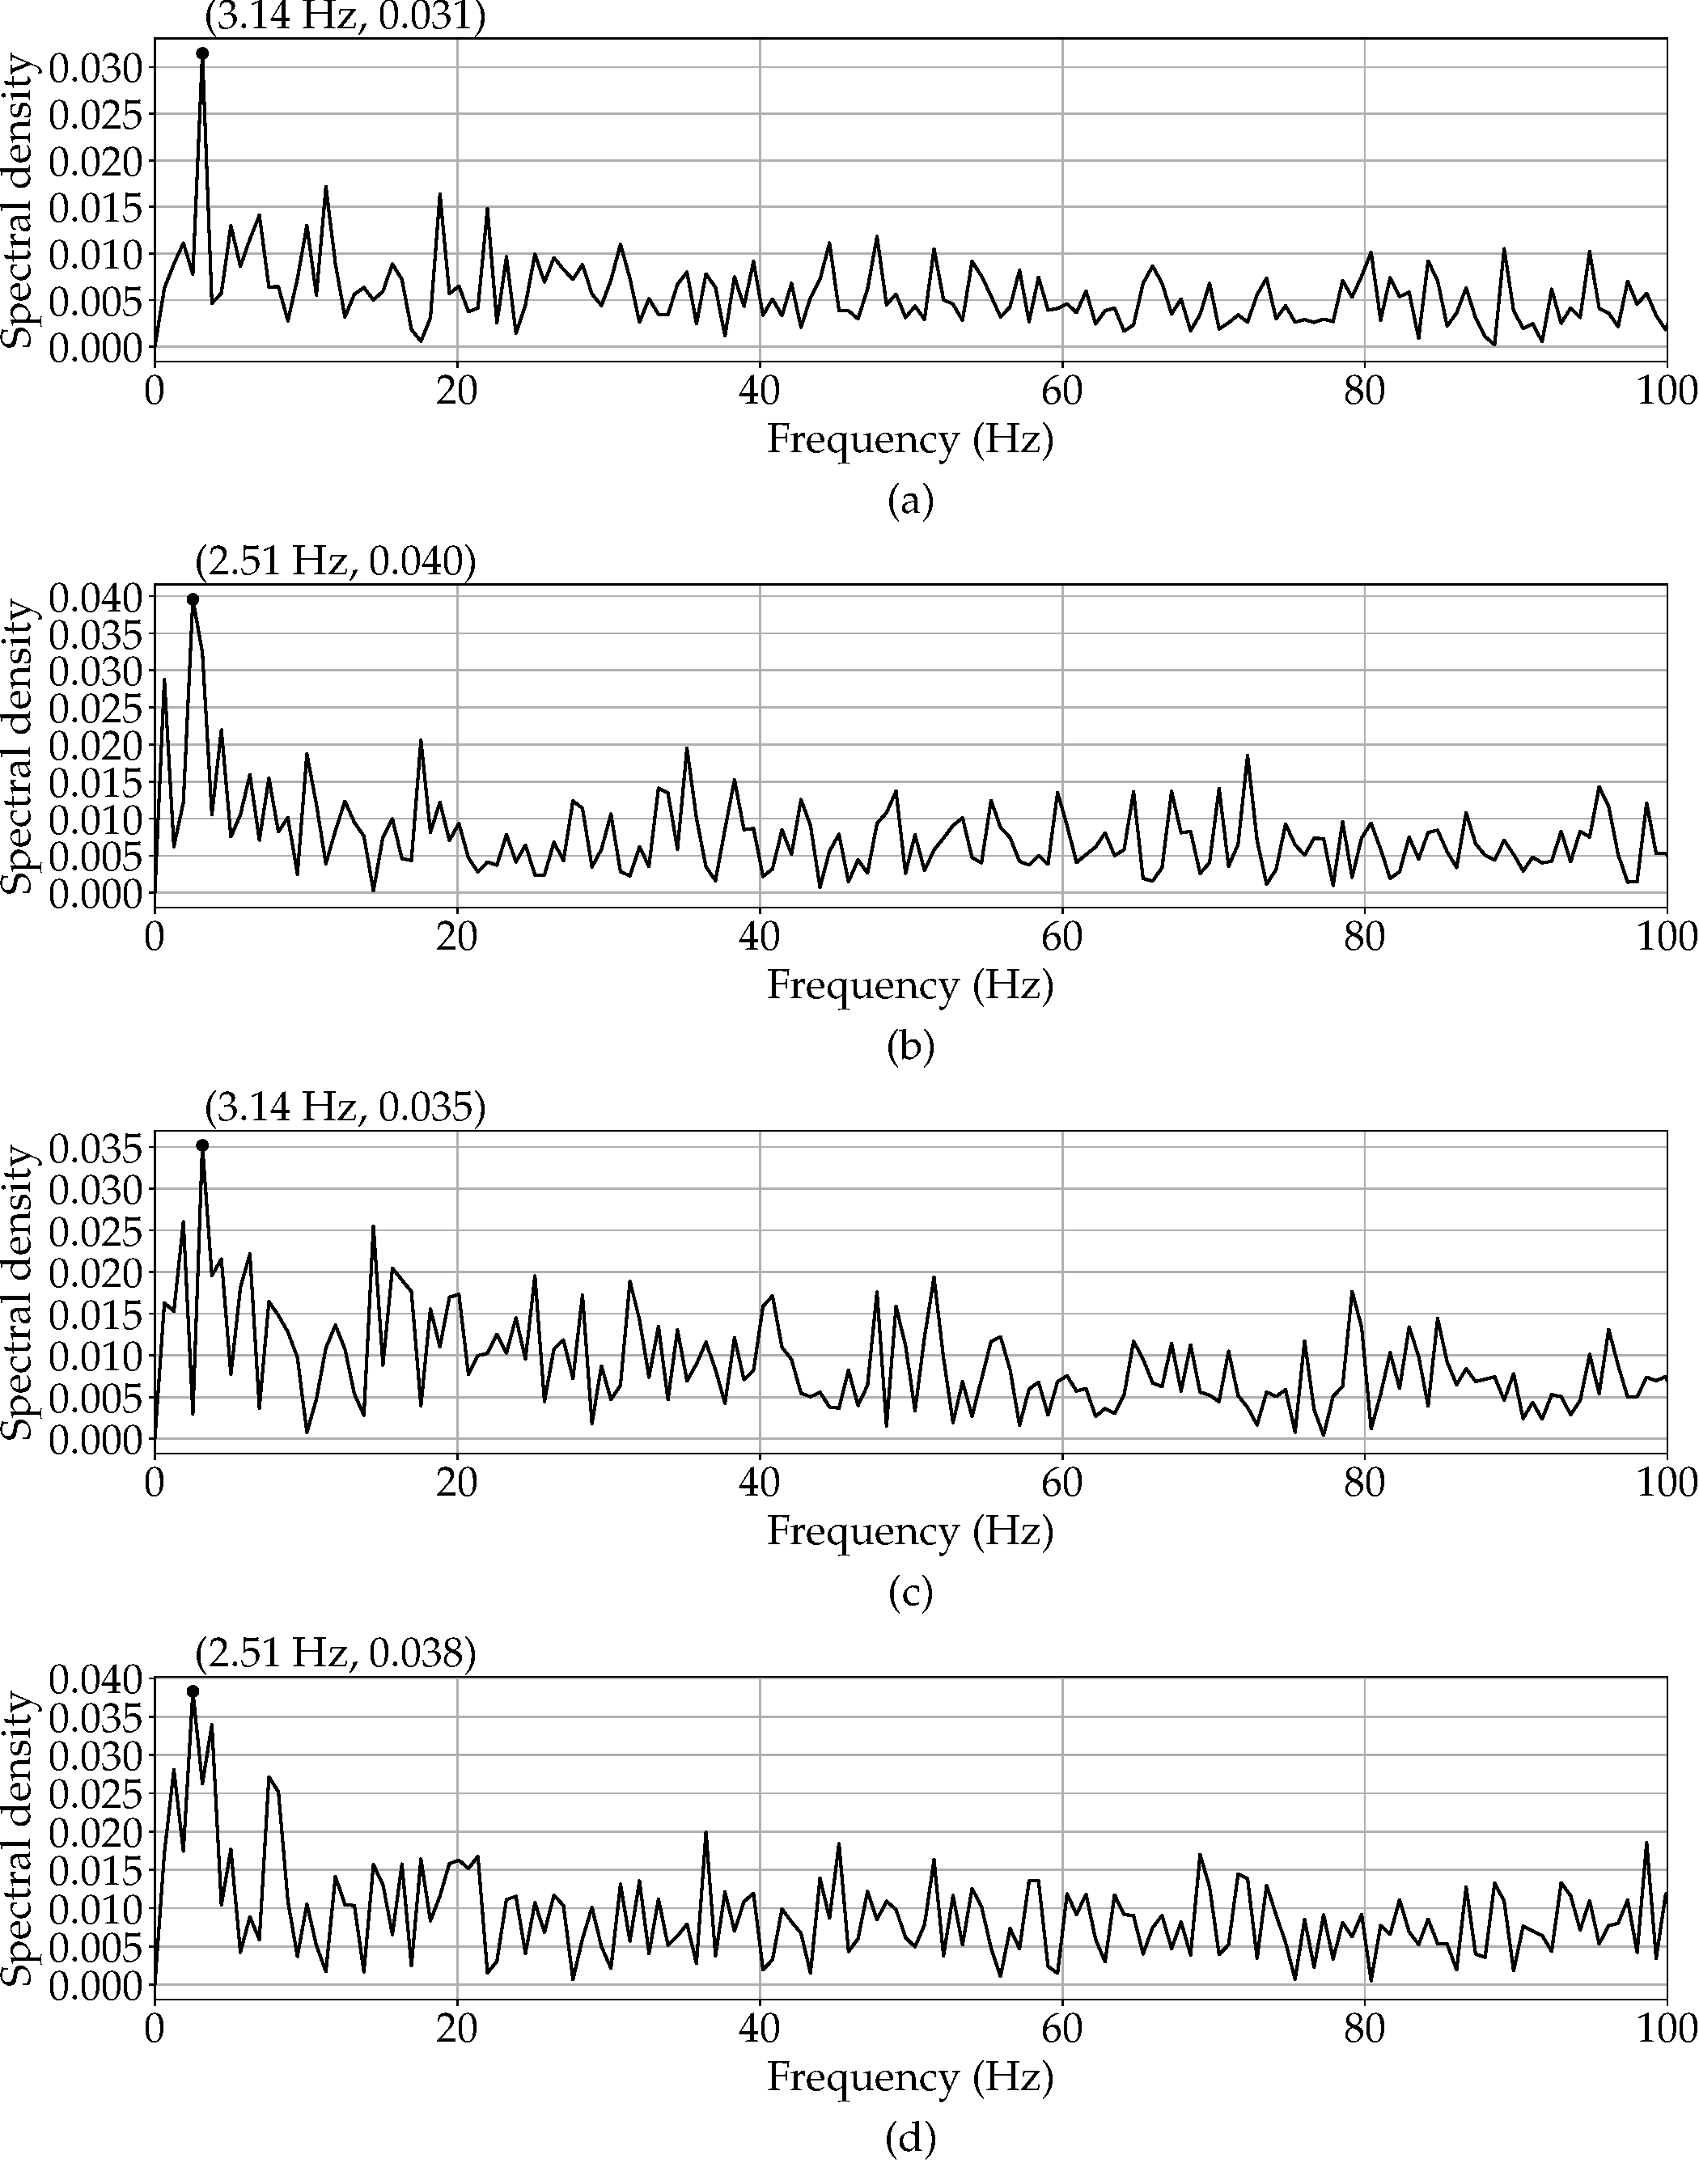
\includegraphics[width=\linewidth]{gfx/FFT_all_freq_x_D_y_0.pdf}
    \caption{Frequency spectral density of velocity for flow Reynolds number (a)~2699, (b)~3818, (c)~4676 and (d)~5399 at a distance of $D$ from the center of the cylinder.}
    \label{fig:surface_x_D_y_0}
\end{figure}

It can be seen in Fig.~\ref{fig:surface_x_D_y_0} that at each flow velocity, the peak frequency is different. This is due to the difference in the formation of the vortex at each velocity. At Reynolds numbers 2699 and 4676, the maximum peak occurs at a frequency of 3.14~Hz and at Reynolds numbers 3818 and 5399, the peak is at 2.51~Hz. The Reynolds number is the ratio of inertial forces to viscous forces. It describes whether the flow is laminar or turbulent. Similarly, the Strouhal number ($St$) is the ratio of oscillatory inertial forces to steady inertial force. It describes the relationship between an unsteady phenomenon (vortex shedding) and flow velocity. The Strouhal number is defined as
\begin{equation}\label{strouhal number}
    St = \frac{f\cdot D}{U},
\end{equation}
where $f$ is the frequency of the vortex in $Hz$, $D$ is the diameter of the solid cylinder and $U$ is the flow velocity. Assuming that the peak frequency in Fig.~\ref{fig:surface_x_D_y_0} dominates the entire spectrum, the peak frequency for all flows is used to calculate the Strouhal number. The two non-dimensional numbers (Reynolds number and Strouhal number) are plotted against each other in Fig.~\ref{fig:st_vs_re_x_D_y_0}. 
\begin{figure}
    \centering
    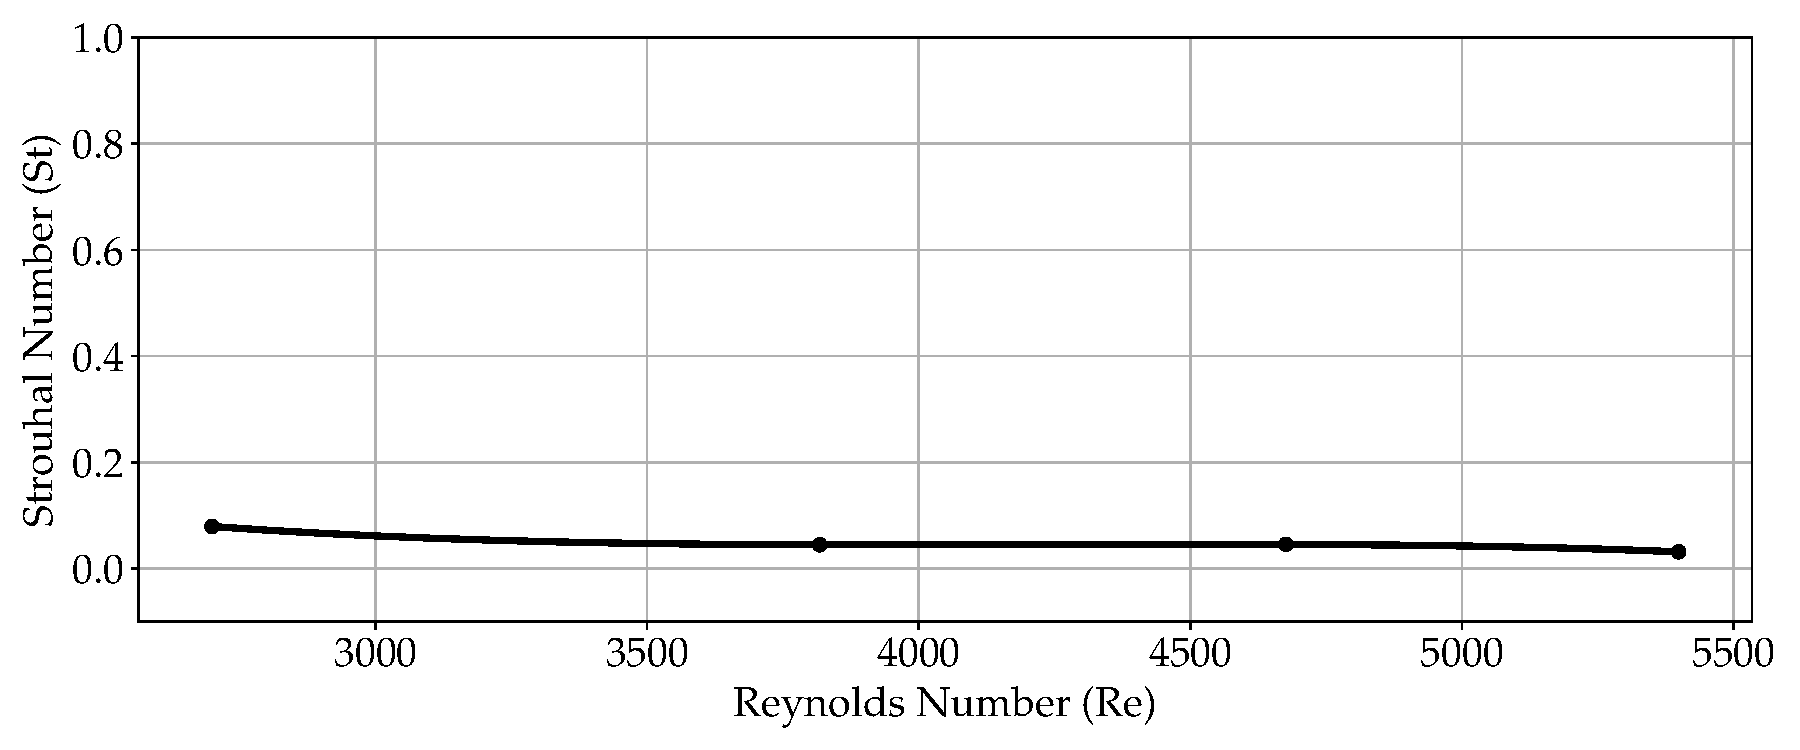
\includegraphics[width=\linewidth]{gfx/Re_vs_St_x_D_y_0.pdf}
    \caption{Variation of Strouhal number ($St$) with Reynolds number ($Re$) for flow past a cylinder at a distance of \enquote{$D$} from the center.}
    \label{fig:st_vs_re_x_D_y_0}
\end{figure}
In the figure, it can be seen that the Strouhal number is decreasing slightly with Reynolds number. This is because the frequency of the vortex decreases with an increase in flow velocity.  The next section discusses the vortex analysis at a distance of $D$ and a height of $0.5~D$ from the center of the cylinder.

\subsection{Vortex analysis at a height of \texorpdfstring{$0.5~D$}~~from the center of the cylinder}

The hot wire anemometer is moved to a height of $0.5~D$ from the center of the cylinder and analysis is performed for four flow speeds having differential pressure of $1~Pa$, $2~Pa$, $3~Pa$ and $4~Pa$. Here, for each flow velocity, the voltage output is measured in the oscilloscope. The corresponding velocity is calculated from the calibration equation (Eq.~(\ref{eq:calib_eqn_hwa})). The velocity is then transformed from the temporal domain to the frequency domain using the Fourier transform equation (Eq.~(\ref{eq:forward fourier})). A comparison of velocity spectral density with frequency for all flow velocities is shown in Fig.~\ref{fig:surface_x_D_y_0-5_D}.
\begin{figure}
    \centering
    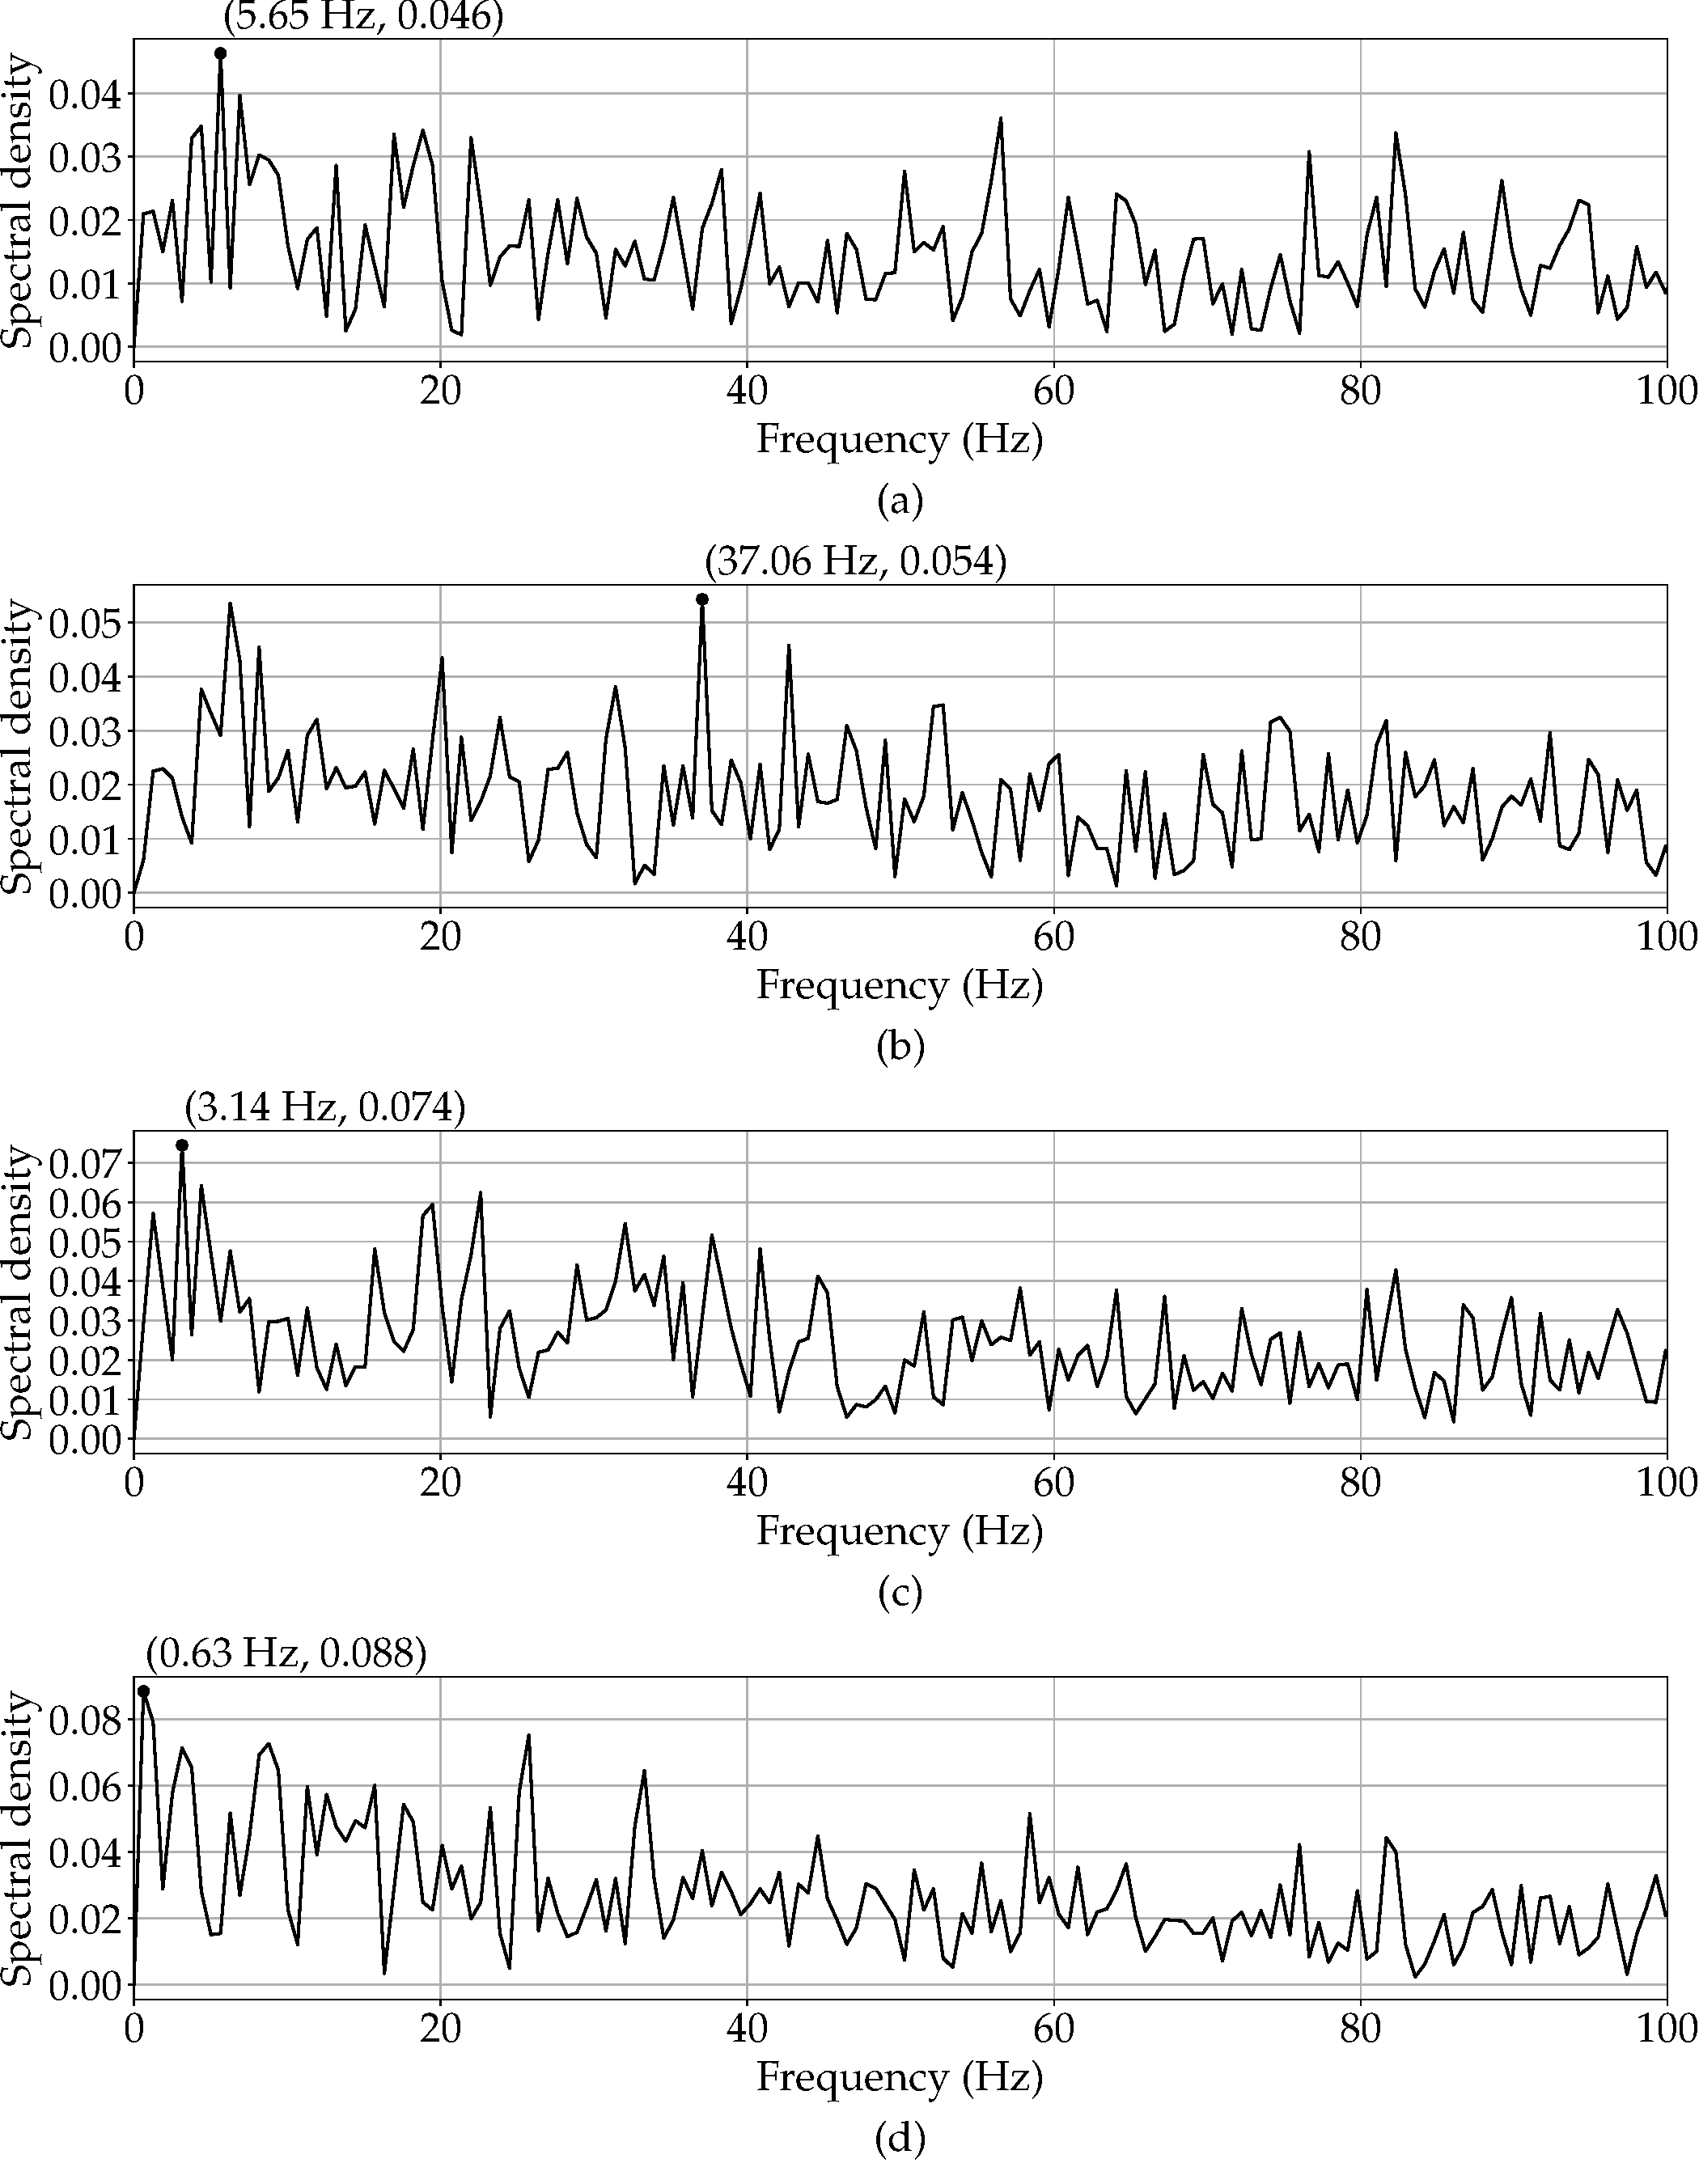
\includegraphics[width=\linewidth]{gfx/FFT_all_freq_x_D_y_0-5_D.pdf}
    \caption{Frequency spectral density of velocity for flow Reynolds number (a)~2699, (b)~3818, (c)~4676 and (d)~5399 at a distance of \enquote{$D$} and a height of \enquote{$0.5~D$} from the center of the cylinder.}
    \label{fig:surface_x_D_y_0-5_D}
\end{figure}
In the figure, it can be seen that the peak frequency for each flow velocity is different from the peak obtained previously. For $Re = 2699$, the peak frequency is 5.65~Hz, for $Re = 3818$, peak frequency is at 37.06~Hz, for $Re = 4676$, the peak frequency is 3.14~Hz and for $Re = 5399$, the peak frequency is 0.63~Hz. These peak frequencies are then used to calculate the Strouhal number (Eq.~(\ref{strouhal number})). The Strouhal number variation with Reynolds number is shown in Fig.~\ref{fig:st_vs_re_x_D_y_0-5_D}. Here, it can be seen that the Strouhal number fluctuates highly in the region of $Re=3000$ to $Re = 4500$. This indicates a change of vortex shedding characteristics when the flow is in transition toward turbulence. The next section discusses the vortex shedding characteristics at a distance of $2~D$ from the center of the cylinder.

\begin{figure}
    \centering
    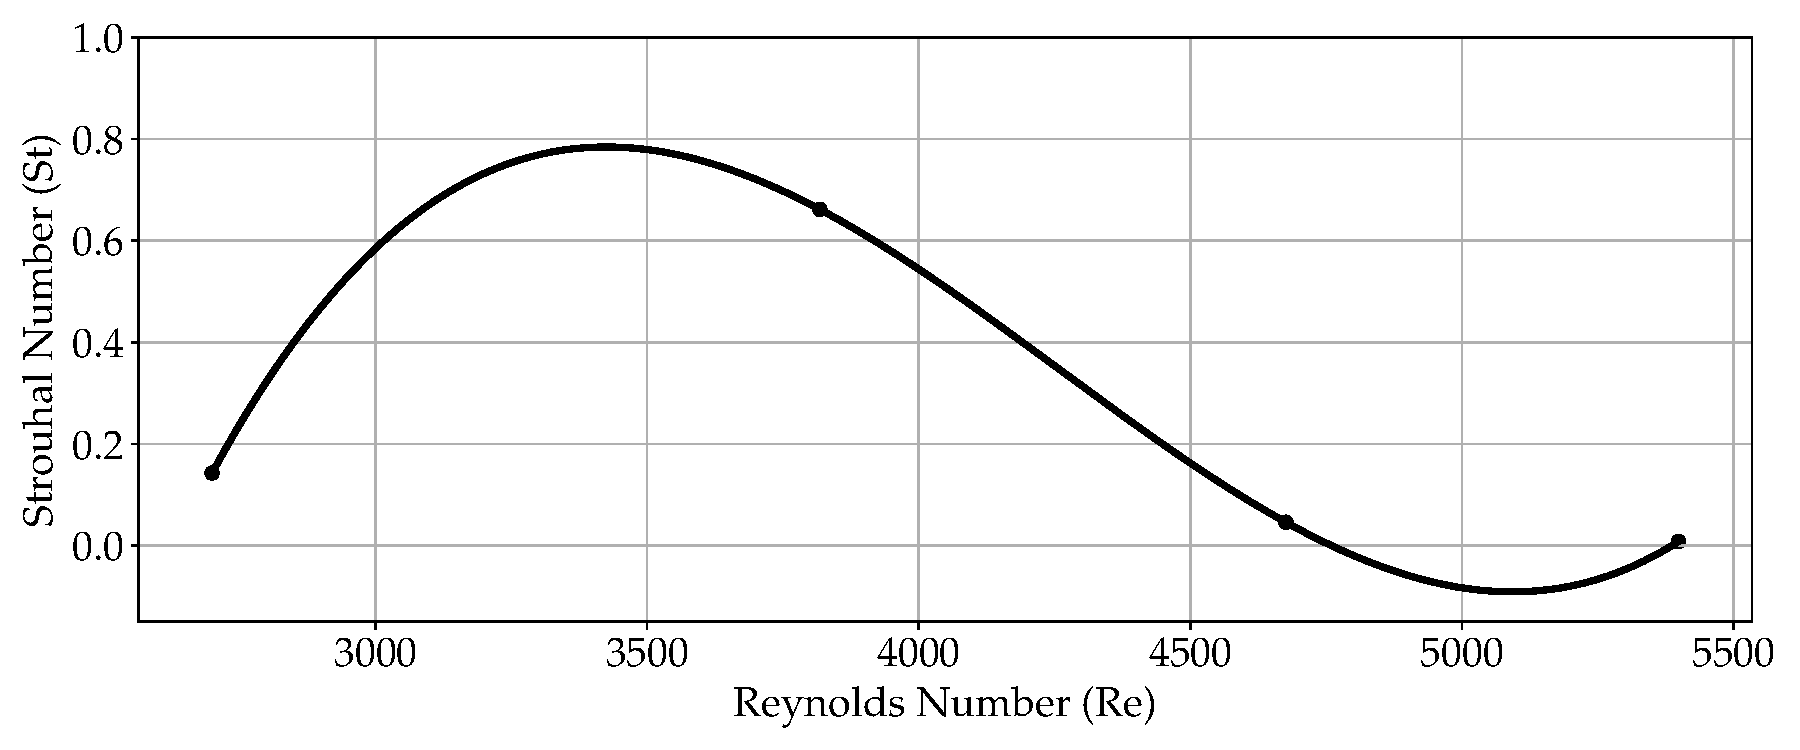
\includegraphics[width=\linewidth]{gfx/Re_vs_St_x_D_y_0-5_D.pdf}
    \caption{Variation of Strouhal number ($St$) with Reynolds number ($Re$) for flow past a cylinder at a distance of \enquote{$D$} and at a height of \enquote{$0.5~D$} from the center of the cylinder.}
    \label{fig:st_vs_re_x_D_y_0-5_D}
\end{figure}

\section{Vortex analysis at distance \texorpdfstring{$x=2D$}~~from the cylinder}
In this section, the vortex shedding characteristics at a distance of $2~D$ from the cylinder is discussed. The analysis is carried out at the center of the cylinder and at a height of $0.5~D$ from the cylinder.
\subsection{Vortex analysis at the center of the cylinder}
The hot wire anemometer is kept at a distance of $2~D$ downstream of the cylinder and the vortices are analyzed for air flow having differential pressures of $1~Pa$, $2~Pa$, $3~Pa$ and $4~Pa$. The output voltage is measured using an oscilloscope and the corresponding velocity is calculated using the calibration equation (Eq.~(\ref{eq:calib_eqn_hwa})). The velocity is transformed from the temporal domain to the frequency domain using Fourier transform (Eq.~(\ref{eq:forward fourier}).  A comparison of velocity spectral density with frequency for all flow velocities is shown in Fig.~\ref{fig:surface_x_2D_y_0}. It can be seen that for $Re = 2699$, the peak frequency is 19.47~Hz, for $Re = 3818$, peak frequency is at 3.77~Hz, for $Re = 4676$, the peak frequency is 0.63~Hz and for $Re = 5399$, the peak frequency is 3.77~Hz. Using these peak frequencies, the Strouhal number is calculated. The variation of the Strouhal number with the Reynolds number is shown in Fig.~\ref{fig:st_vs_re_x_2D_y_0}. 
\begin{figure}
    \centering
    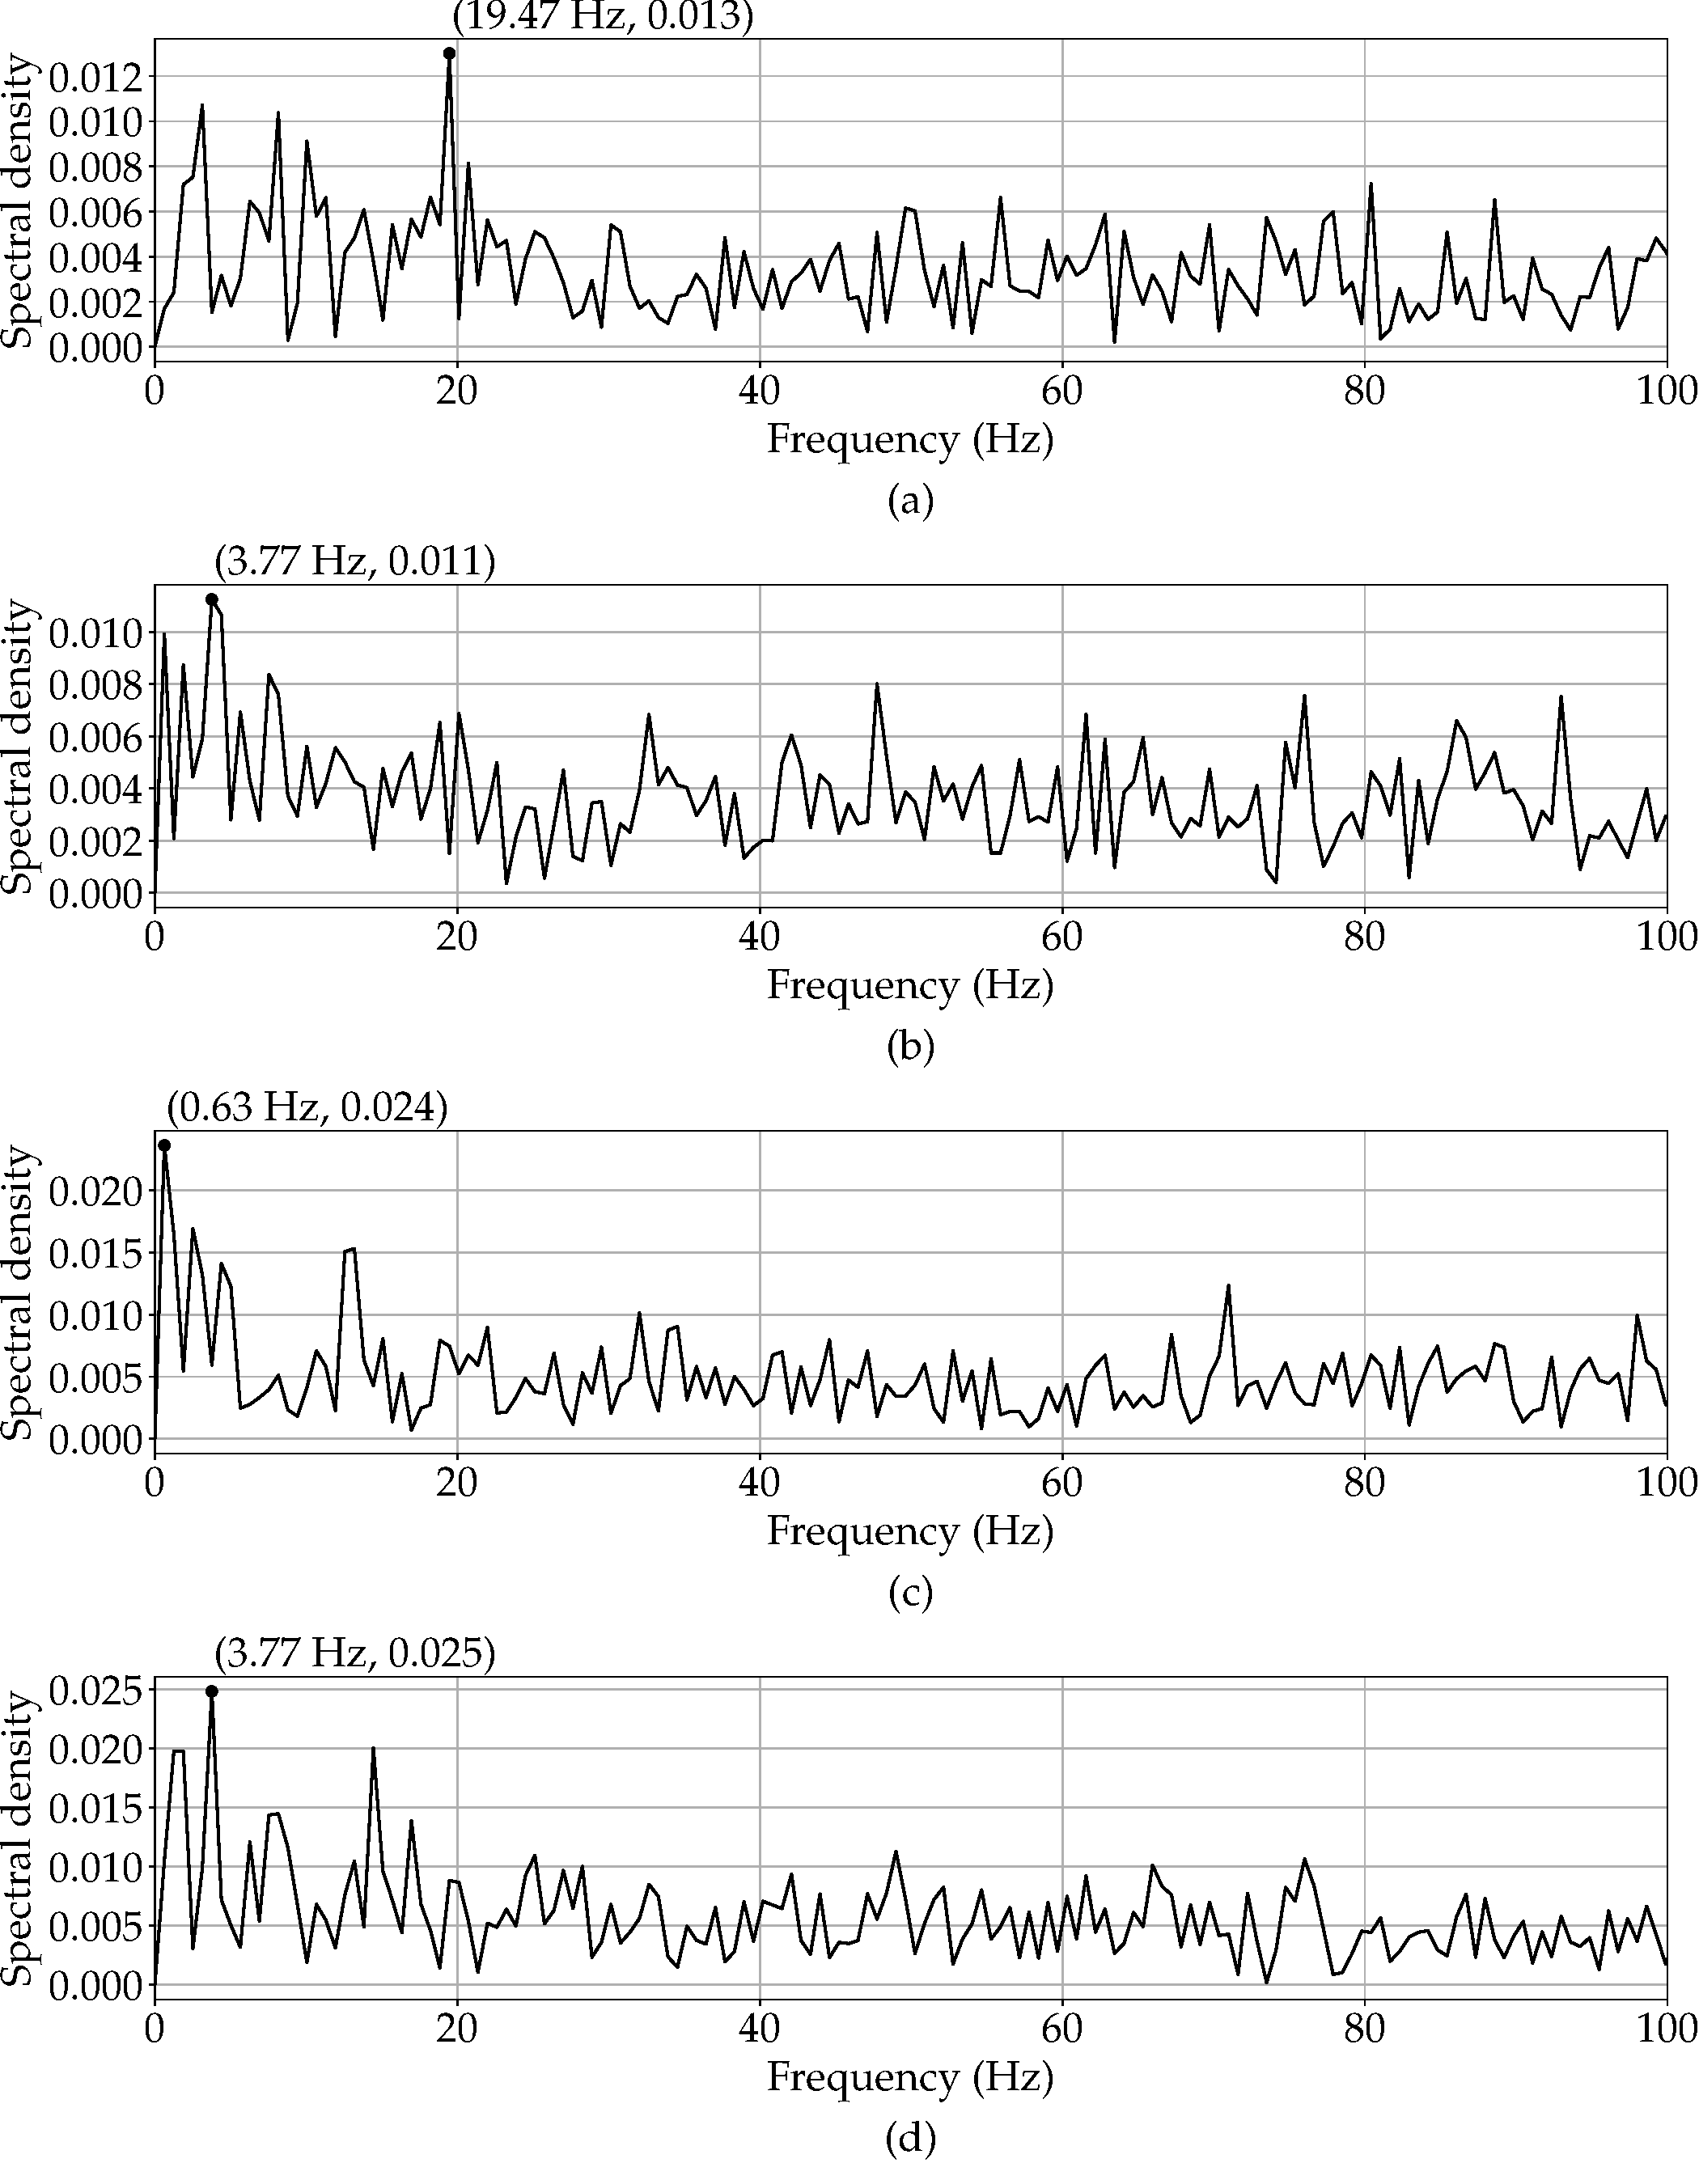
\includegraphics[width=\linewidth]{gfx/FFT_all_freq_x_2D_y_0.pdf}
    \caption{Frequency spectral density of velocity for flow Reynolds number (a)~2699, (b)~3818, (c)~4676 and (d)~5399 at a distance of \enquote{$2~D$} from the center of the cylinder.}
    \label{fig:surface_x_2D_y_0}
\end{figure}

\begin{figure}
    \centering
    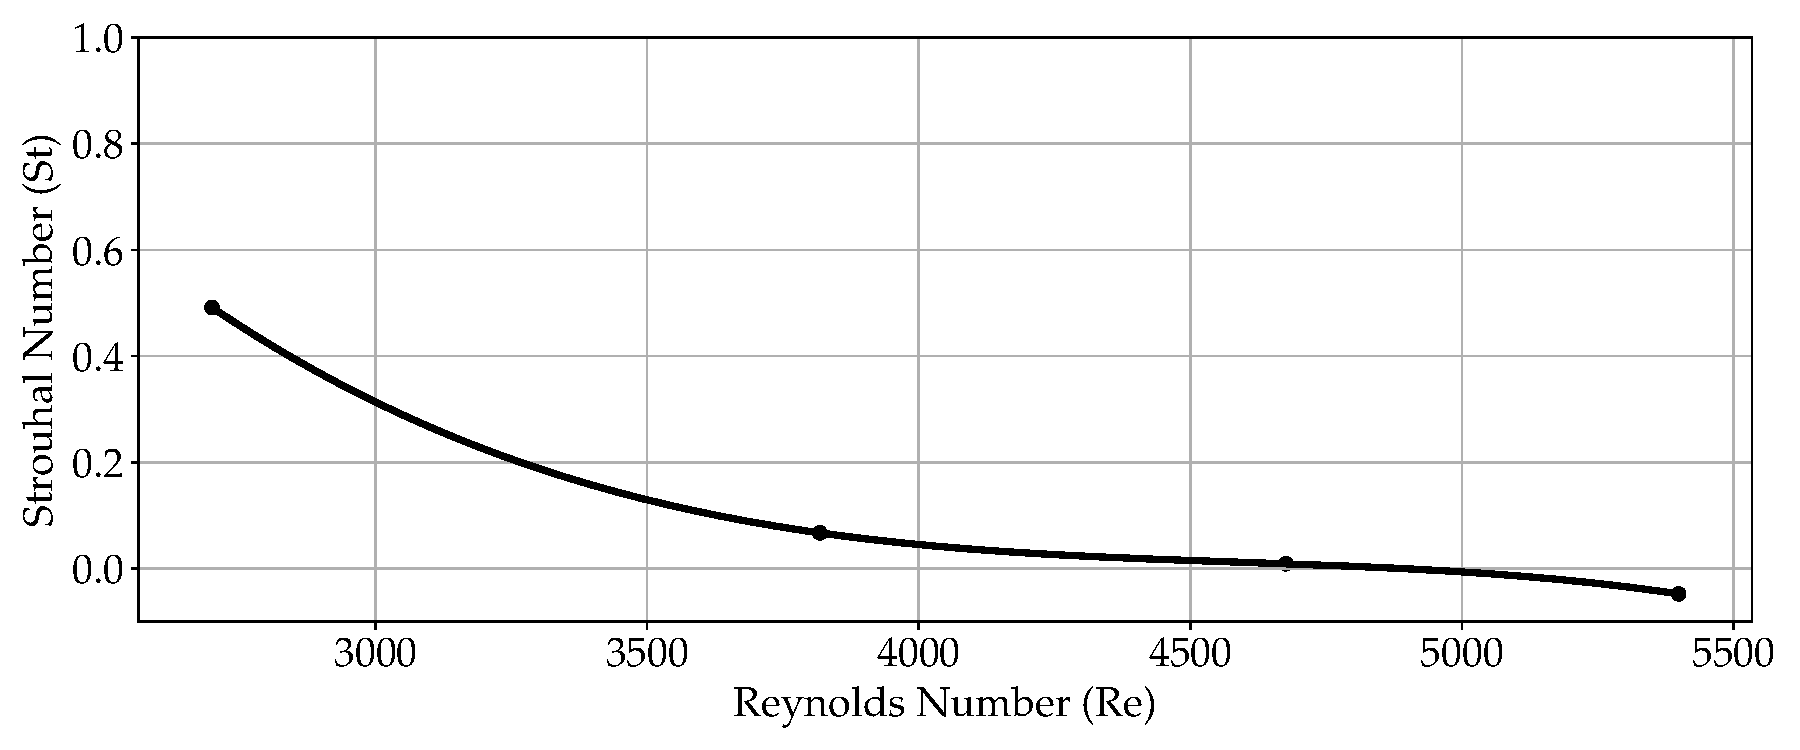
\includegraphics[width=\linewidth]{gfx/Re_vs_St_x_2D_y_0.pdf}
    \caption{Variation of Strouhal number ($St$) with Reynolds number ($Re$) for flow past a cylinder at a distance of \enquote{$2~D$} from the center of the cylinder.}
    \label{fig:st_vs_re_x_2D_y_0}
\end{figure}
In Fig.~\ref{fig:st_vs_re_x_2D_y_0}, it can be seen that the Strouhal number decreases with an increase in the Reynolds number. This is because of the reduction of the frequency of vortices with increase in velocity.

\subsection{Vortex analysis at a height of \texorpdfstring{$0.5~D$}~~from the center of the cylinder}

The hot wire anemometer is then moved to a height of $0.5~D$ from the center of the cylinder and the analysis is performed again for the four flow speeds with differential pressures of $1~Pa$, $2~Pa$, $3~Pa$ and $4~Pa$. For each flow velocity, the voltage output from the hot wire anemometer is measured in the oscilloscope. The velocities corresponding to the voltages are calculated from the calibration equation (Eq.~(\ref{eq:calib_eqn_hwa})). Then it is transformed from the temporal domain to the frequency domain using the Fourier transform equation (Eq.~(\ref{eq:forward fourier})). A comparison of velocity spectral density with frequency for all flow velocities is shown in Fig.~\ref{fig:surface_x_2D_y_0-5_D}.

\begin{figure}
    \centering
    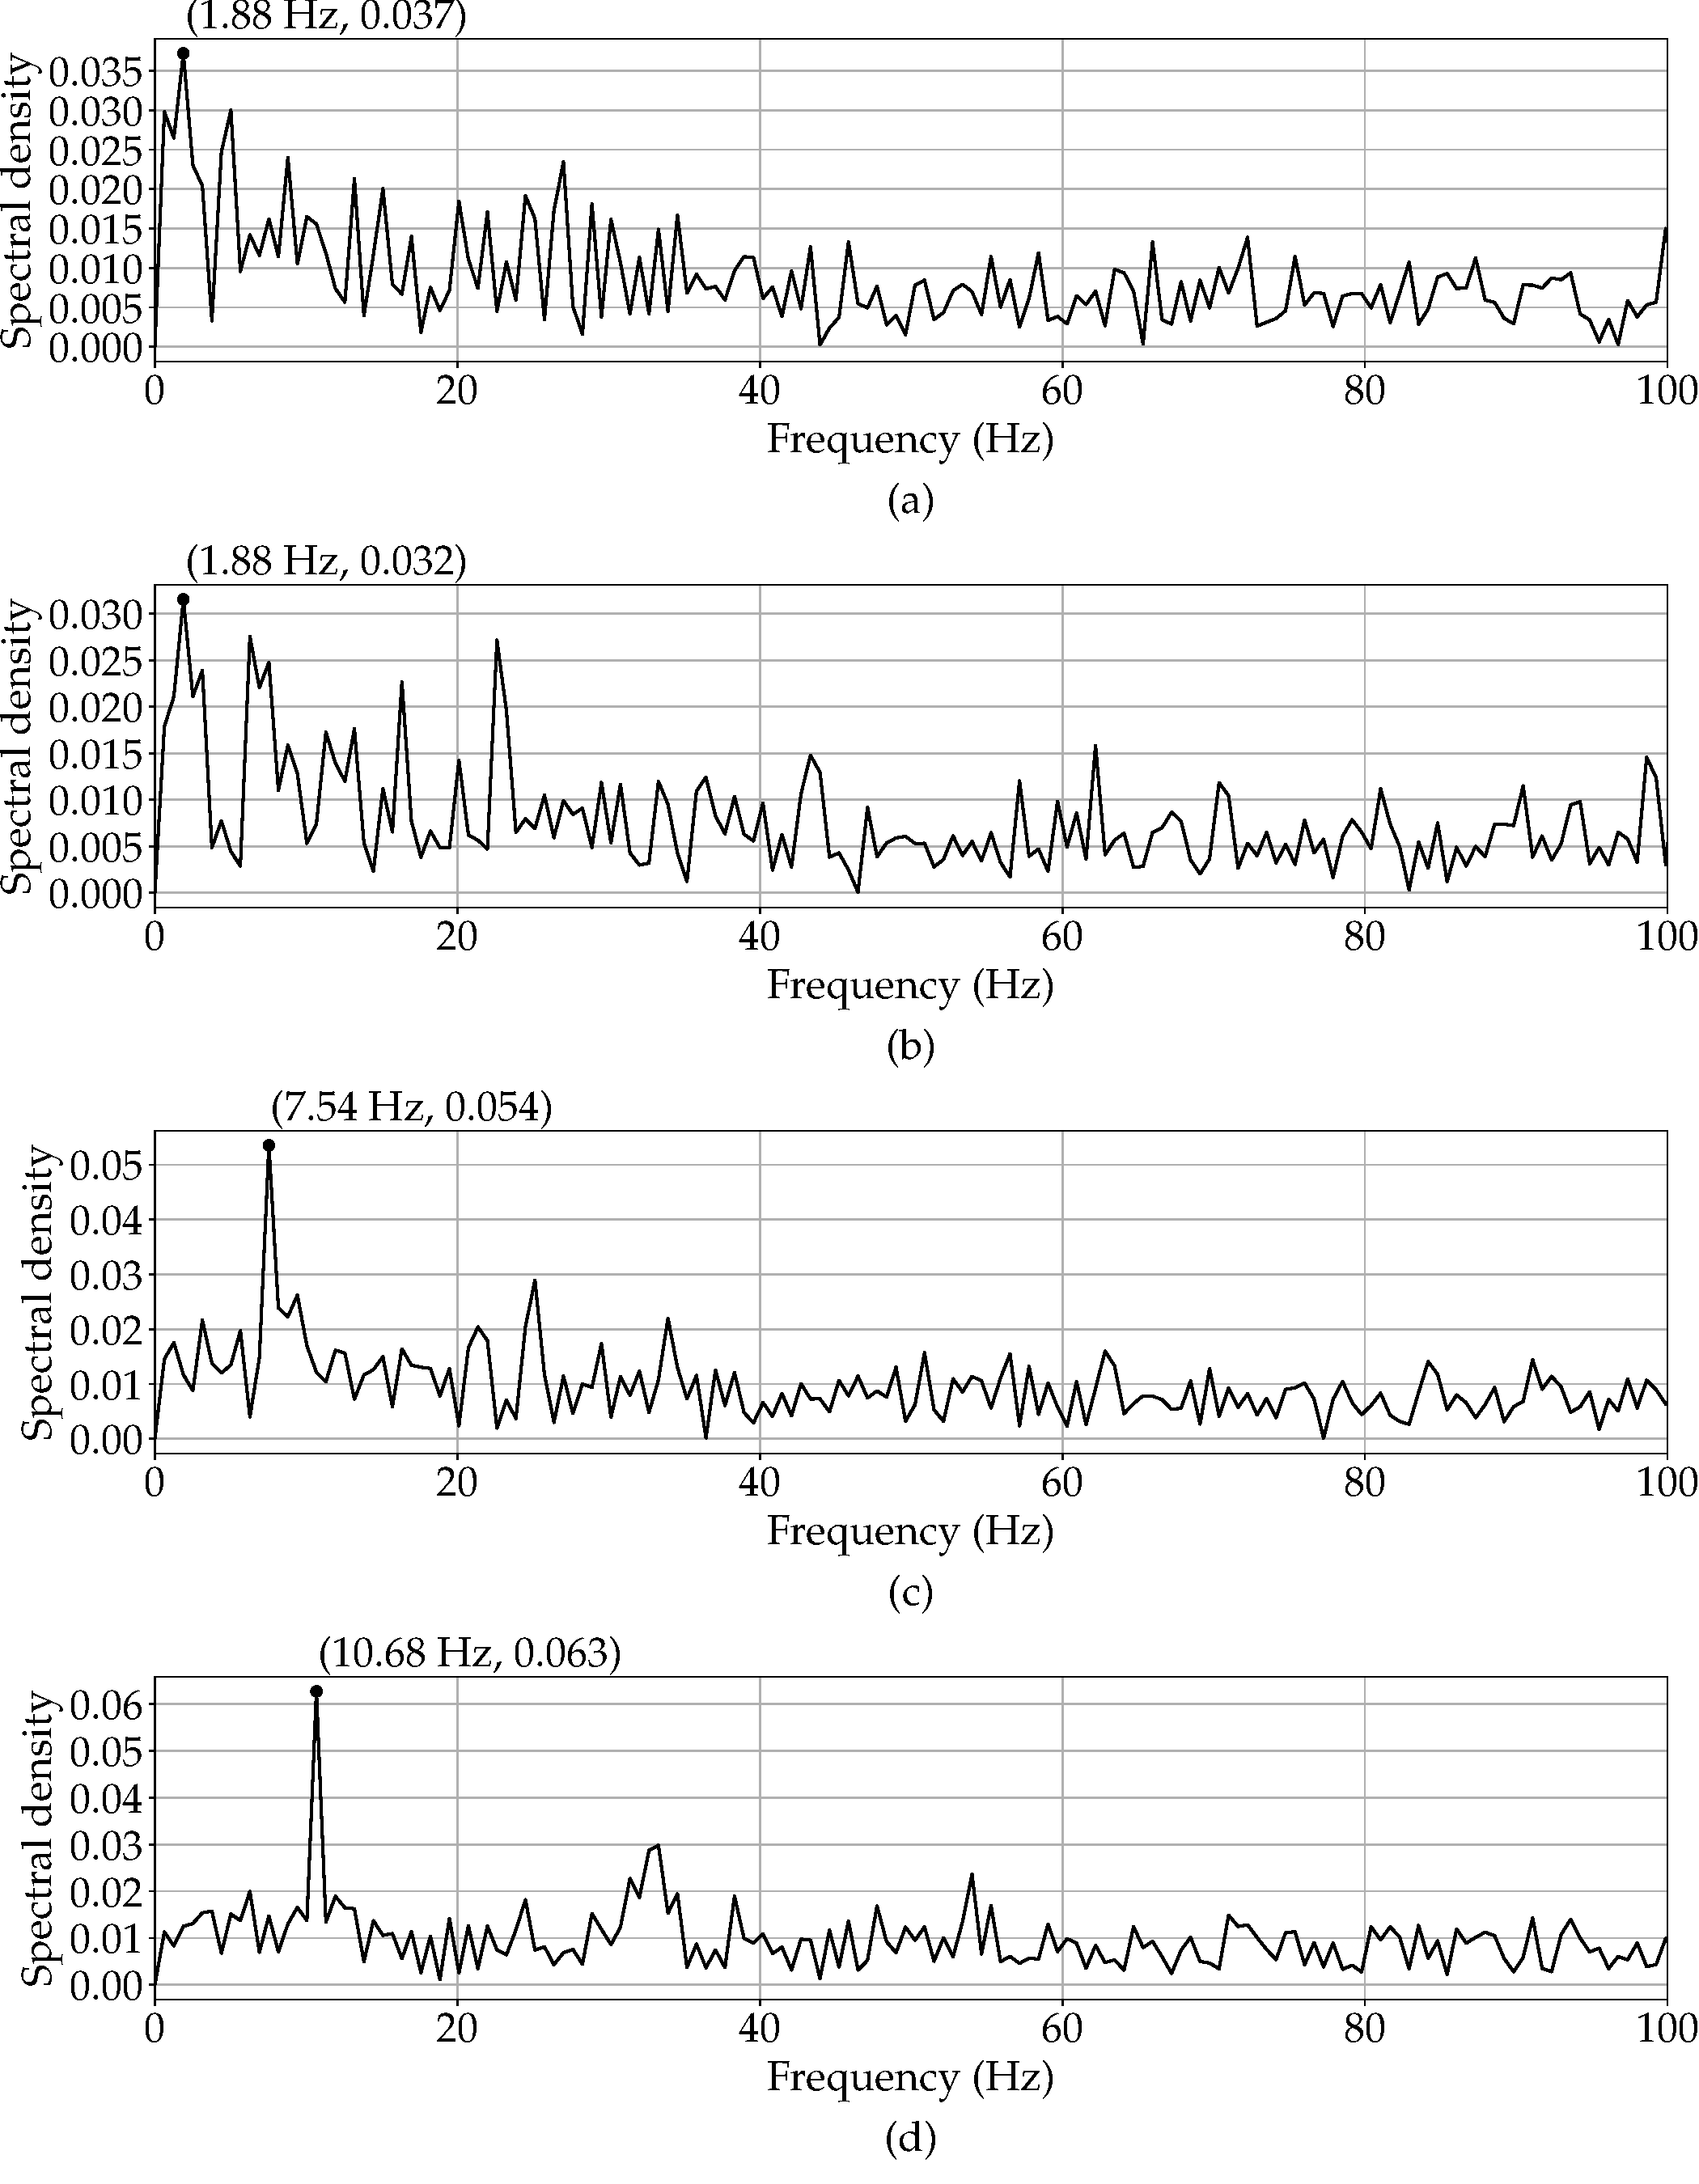
\includegraphics[width=\linewidth]{gfx/FFT_all_freq_x_2D_y_0-5_D.pdf}
    \caption{Frequency spectral density of velocity for flow Reynolds number (a)~2699, (b)~3818, (c)~4676 and (d)~5399 at a distance of \enquote{2~D} and a height of \enquote{0.5~D} from the center of the cylinder.}
    \label{fig:surface_x_2D_y_0-5_D}
\end{figure}

The peak frequencies are 1.88~Hz for $Re = 2699$, 1.88~Hz for $Re = 3818$, 7.54~Hz for $Re = 4676$ and 10.68~Hz for $Re = 5399$. These peak frequencies are used to calculate the Strouhal number (Eq.~(\ref{strouhal number})) and is plotted against the Reynolds number. The comparison between the Reynolds number and the Strouhal number is shown in Fig.~\ref{fig:st_vs_re_x_2D_y_0-5_D}. 
\begin{figure}
    \centering
    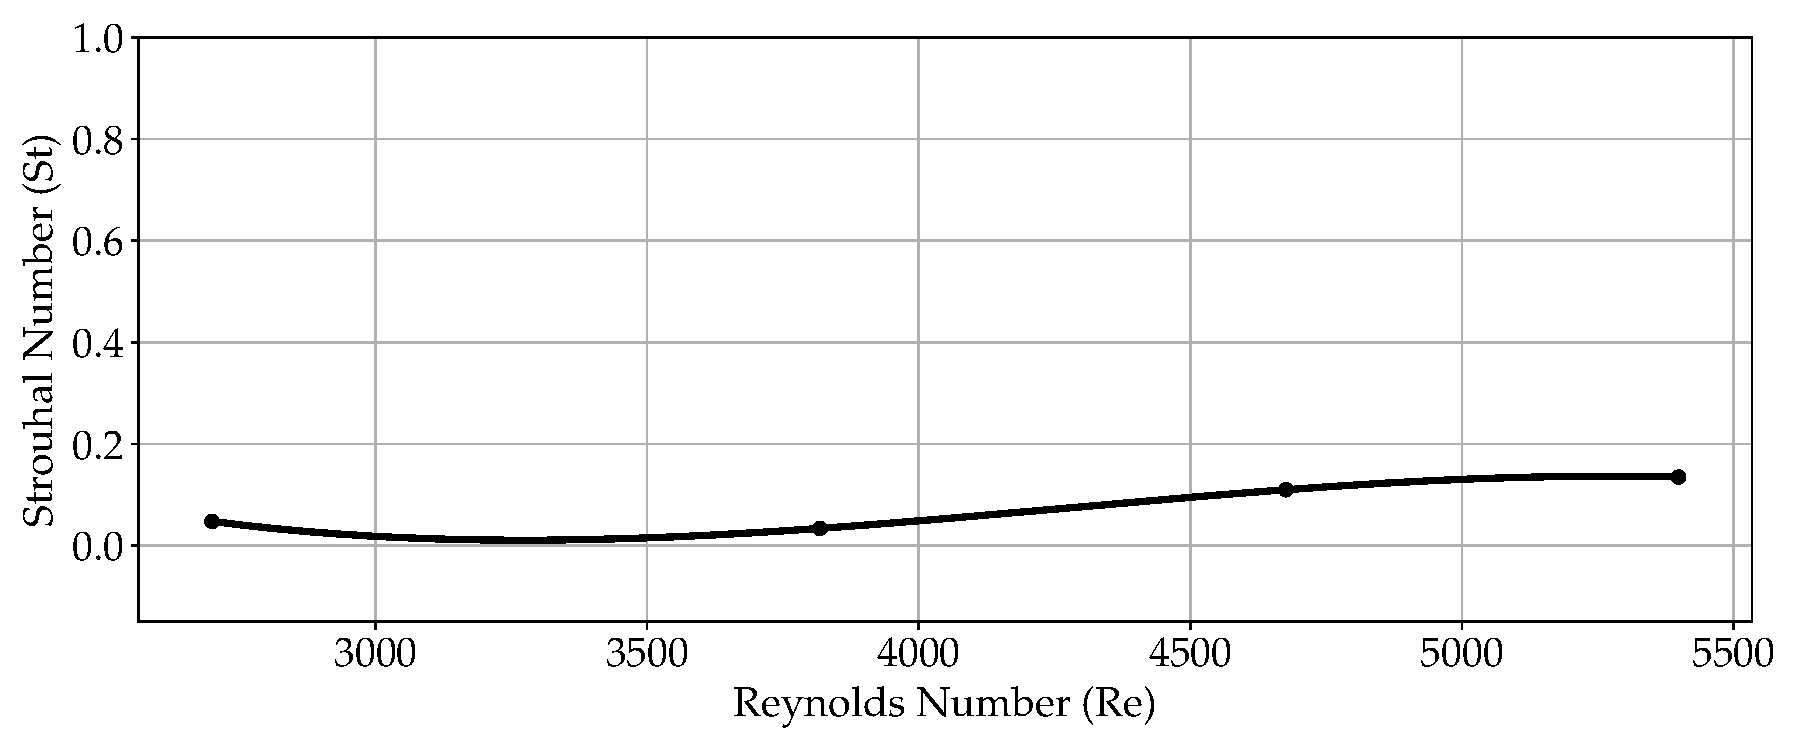
\includegraphics[width=\linewidth]{gfx/Re_vs_St_x_2D_y_0-5_D.pdf}
    \caption{Variation of Strouhal number ($St$) with Reynolds number ($Re$) for flow past a cylinder at a distance of \enquote{$2~D$} and at a height of \enquote{0.5~D} from the center of the cylinder.}
    \label{fig:st_vs_re_x_2D_y_0-5_D}
\end{figure}
Here, the Strouhal number increases with an increase in Reynolds number. This is due to the increase of the vortex frequency when there is an increase in the flow speed. The next section discusses the vortex shedding characteristics at a distance of $4~D$ from the center of the cylinder.

\section{Vortex analysis at distance \texorpdfstring{$x=4D$}~~from the cylinder}
In this section, the vortex analysis is performed at a distance of $4~D$ from the cylinder. The analysis is carried out at the center of the cylinder and at a height of $0.5~D$ from the cylinder.

\subsection{Vortex analysis at the center of the cylinder}
The hot wire anemometer is kept at a distance of $4~D$ downstream of the cylinder and vortex analysis is carried out for air flow having differential pressures of $1~Pa$, $2~Pa$, $3~Pa$ and $4~Pa$. The output voltage across the hot wire anemometer is measured using an oscilloscope and the corresponding velocity is calculated using the calibration equation (Eq.~(\ref{eq:calib_eqn_hwa})). The velocity is transformed from the temporal domain to the frequency domain using Fourier transform (Eq.~(\ref{eq:forward fourier}).  A comparison of velocity spectral density with frequency for all flow velocities is shown in Fig.~\ref{fig:surface_x_4D_y_0}. 
\begin{figure}
    \centering
    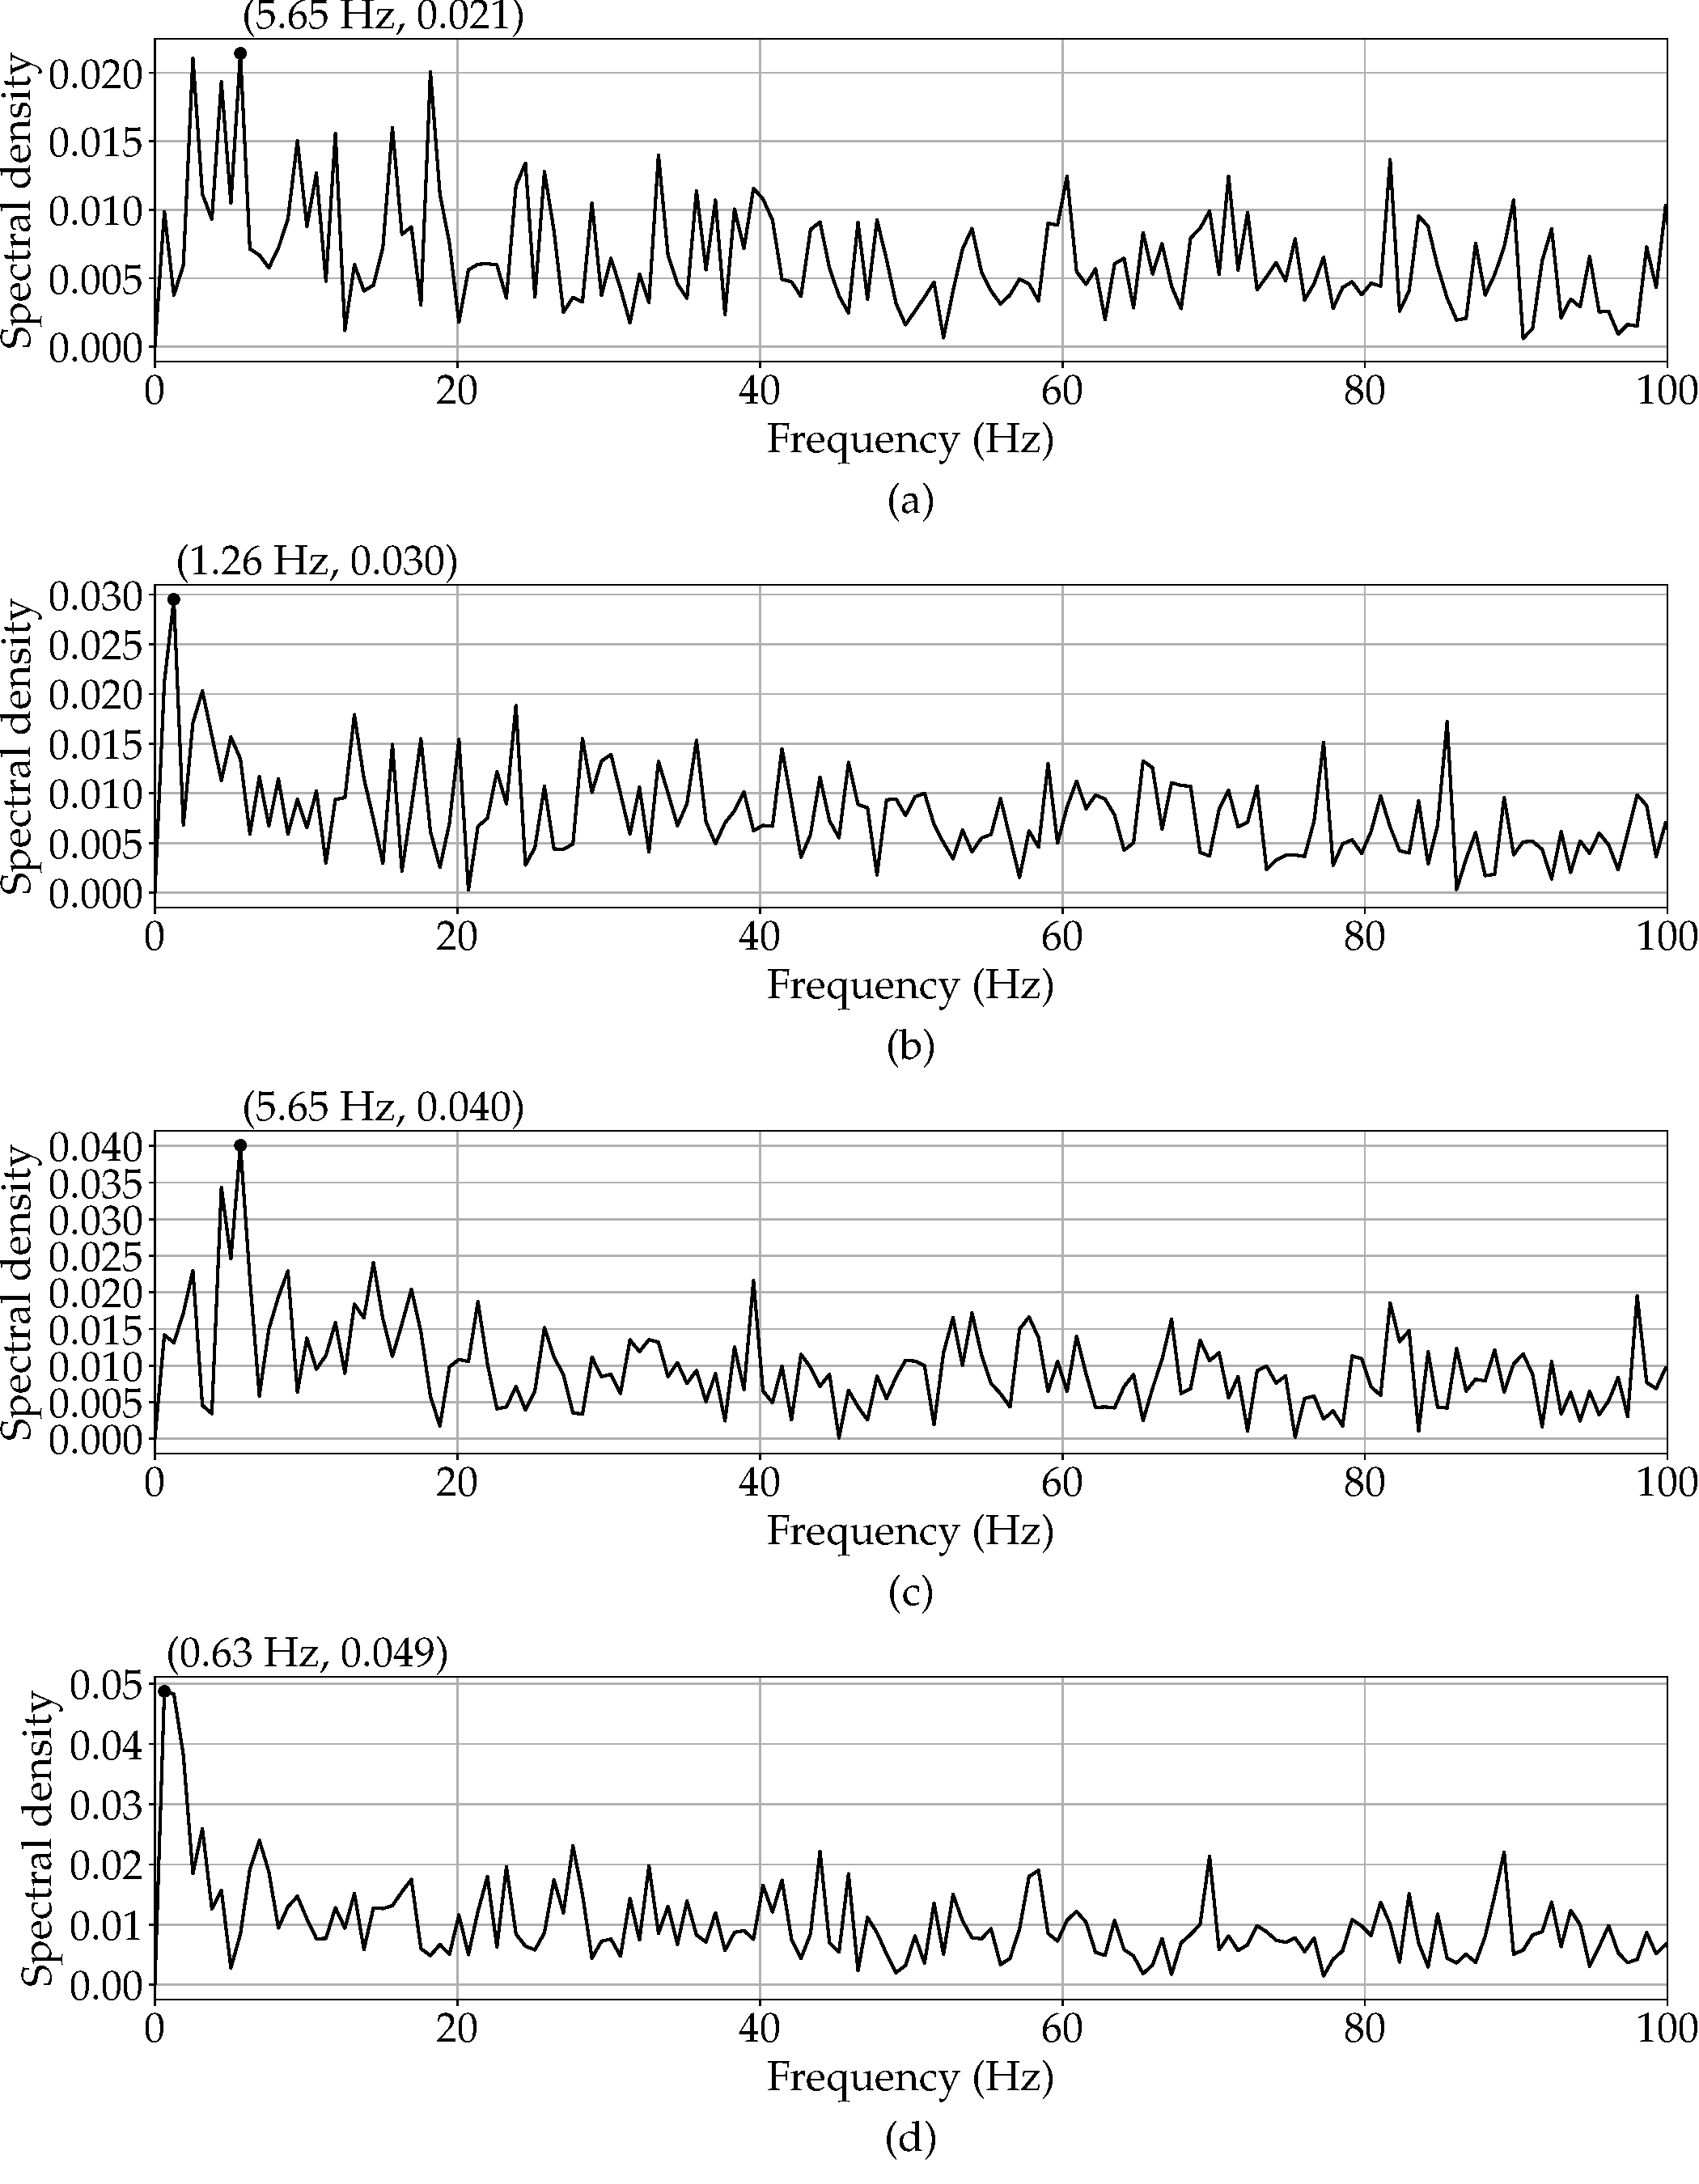
\includegraphics[width=\linewidth]{gfx/FFT_all_freq_x_4D_y_0.pdf}
    \caption{Frequency spectral density of velocity for flow Reynolds number (a)~2699, (b)~3818, (c)~4676 and (d)~5399 at a distance of \enquote{4~D} from the center of the cylinder.}
    \label{fig:surface_x_4D_y_0}
\end{figure}
\begin{figure}
    \centering
    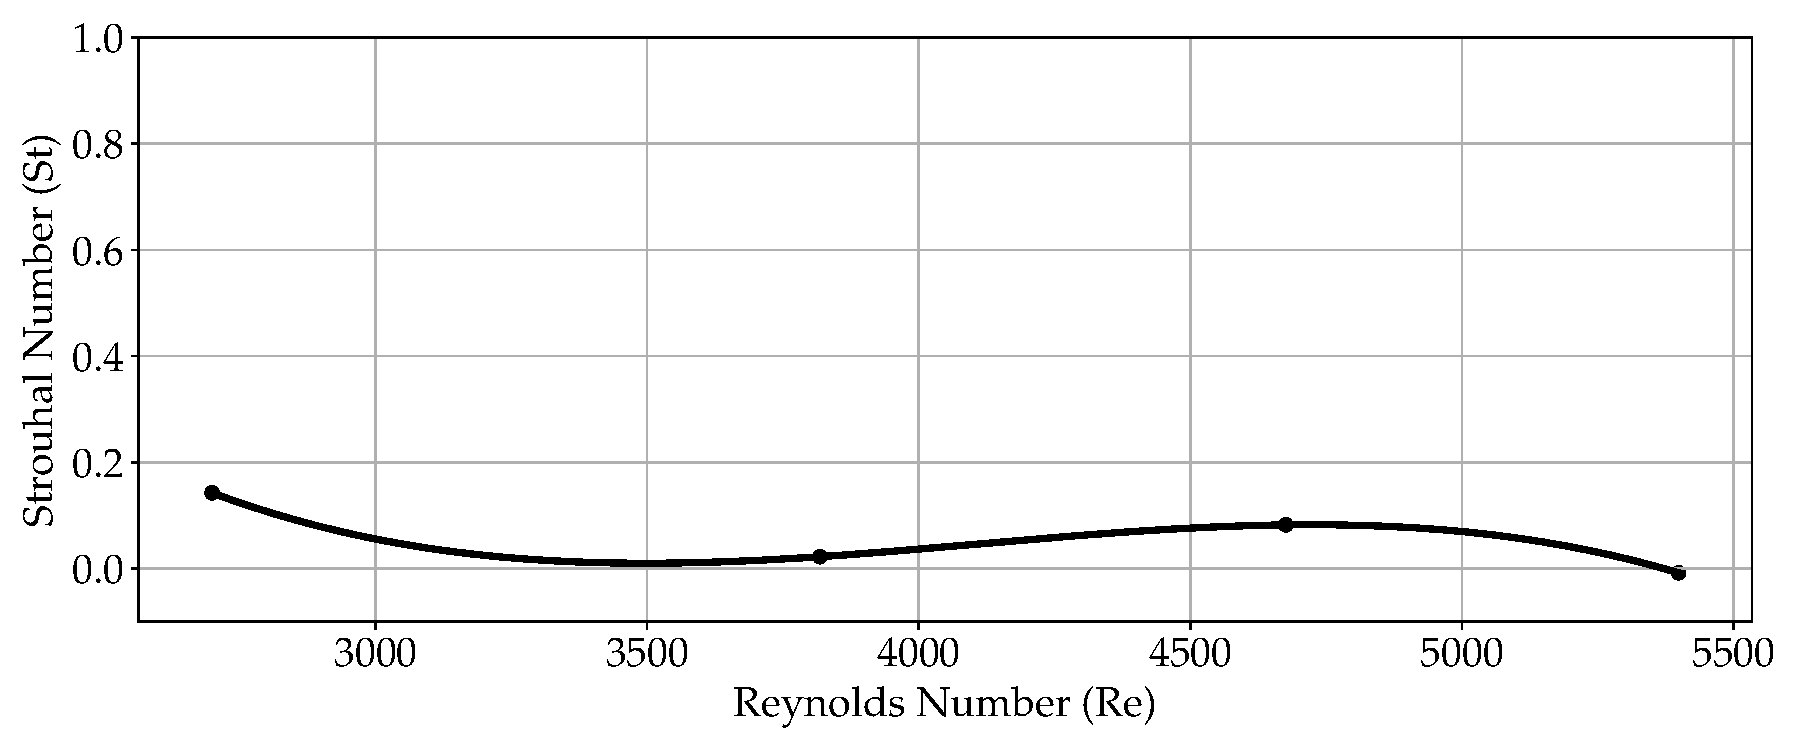
\includegraphics[width=\linewidth]{gfx/Re_vs_St_x_4D_y_0.pdf}
    \caption{Variation of Strouhal number ($St$) with Reynolds number ($Re$) for flow past a cylinder at a distance of \enquote{$4~D$} from the center of the cylinder.}
    \label{fig:st_vs_re_x_4D_y_0}
\end{figure}
It can be seen that for $Re = 2699$, the peak frequency is 5.65~Hz, for $Re = 3818$, peak frequency is at 1.26~Hz, for $Re = 4676$, the peak frequency is 5.65~Hz and for $Re = 5399$, the peak frequency is 0.63~Hz. Using these peak frequencies, the Strouhal number is calculated. The variation of the Strouhal number with the Reynolds number is shown in Fig.~\ref{fig:st_vs_re_x_4D_y_0}. The Strouhal number is in the range 0 to 0.2 which is normal but the low fluctuation is due to its transition towards turbulence.

\subsection{Vortex analysis at a height of \texorpdfstring{$0.5~D$}~~from the center of the cylinder}

The hot wire anemometer is shifted to a height of 0.5~D from the center of the cylinder and vortex analysis is performed for all tow speeds. The voltage output is measured across the sensor in the oscilloscope. The corresponding velocity is calculated from the calibration equation (Eq.~(\ref{eq:calib_eqn_hwa})). The velocity is then transformed from the temporal domain to the frequency domain using the Fourier transform equation (Eq.~(\ref{eq:forward fourier})). A comparison of velocity spectral density with frequency for all flow velocities is shown in Fig.~\ref{fig:surface_x_4D_y_0-5_D}. It can be seen in Fig.~\ref{fig:surface_x_4D_y_0-5_D} that the peak frequencies are 1.26~Hz for $Re = 2699$, 1.26~Hz for $Re = 3818$, 1025.79~Hz for $Re = 4676$ and 1282.71~Hz for $Re = 5399$. The high increase in frequency is due to increased disturbances as the flow is in transition to turbulence. These peak frequencies are used to calculate the Strouhal number (Eq.~(\ref{strouhal number})) and is plotted against the Reynolds number. The comparison between the Reynolds number and the Strouhal number is shown in Fig.~\ref{fig:st_vs_re_x_4D_y_0-5_D}. 
\begin{figure}[H]
    \centering
    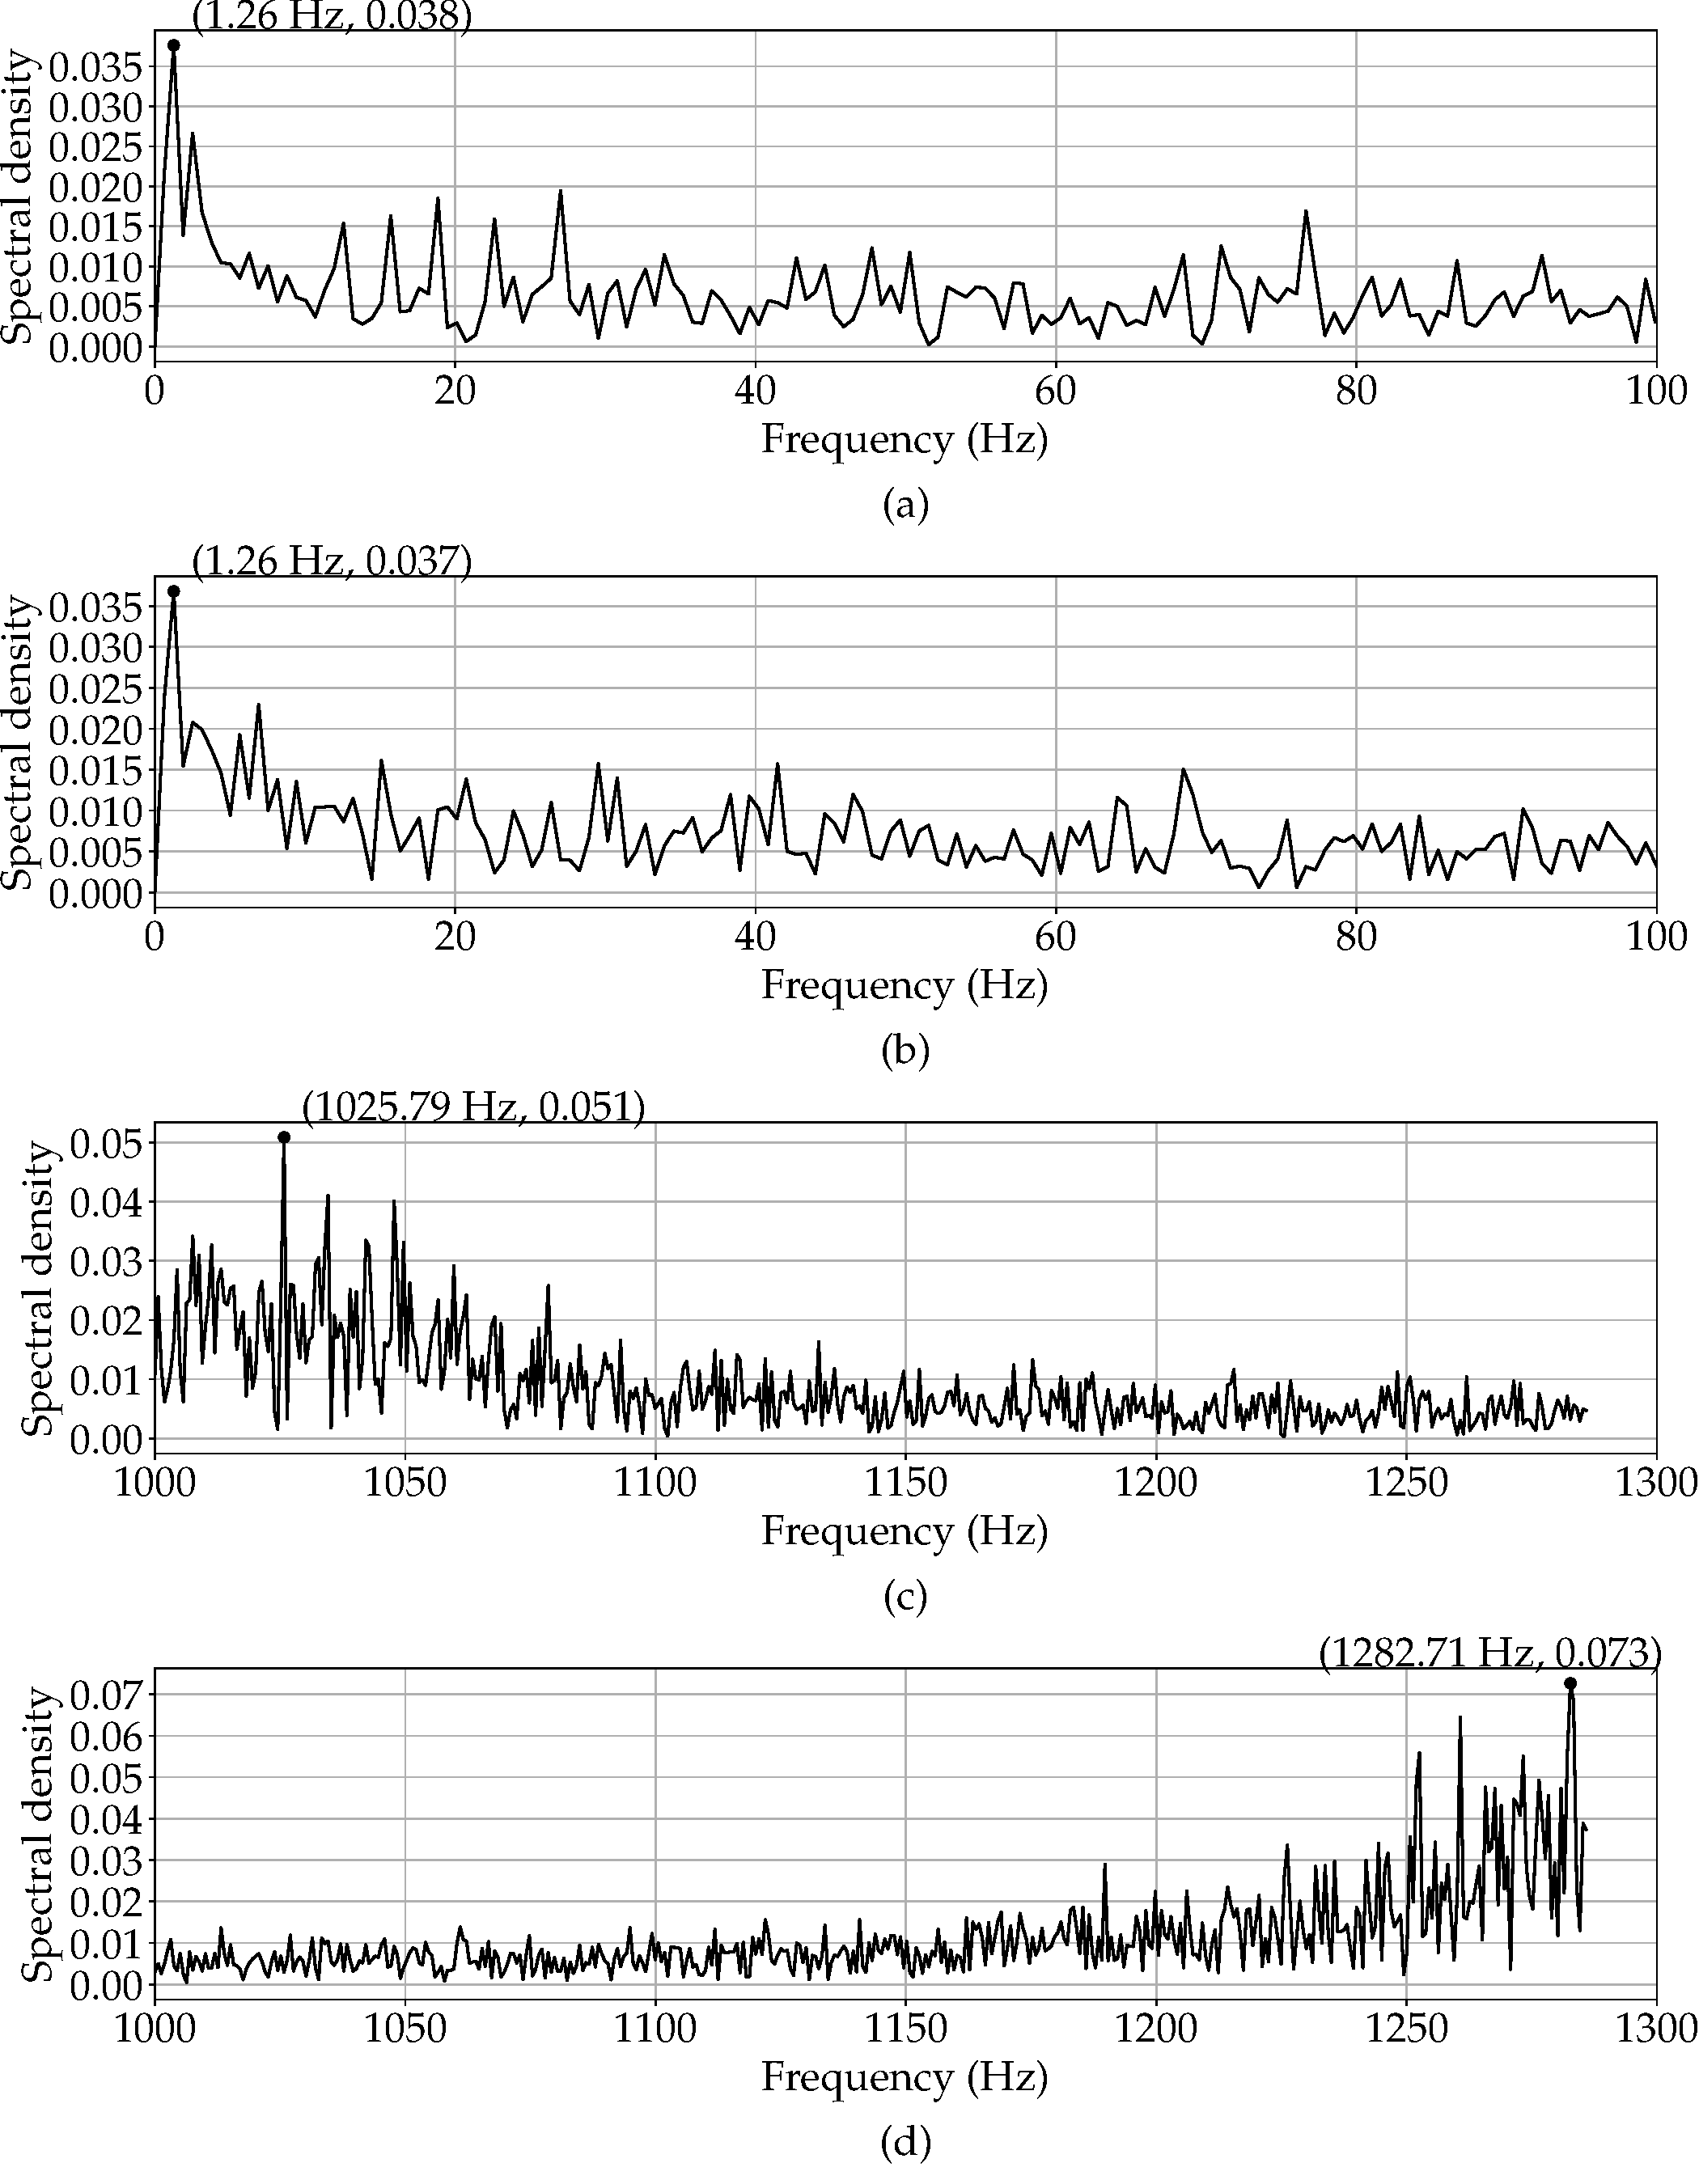
\includegraphics[width=\linewidth]{gfx/FFT_all_freq_x_4D_y_0-5_D.pdf}
    \caption{Frequency spectral density of velocity for flow Reynolds number (a)~2699, (b)~3818, (c)~4676 and (d)~5399 at a distance of \enquote{4~D} and a height of \enquote{0.5~D} from the center of the cylinder.}
    \label{fig:surface_x_4D_y_0-5_D}
\end{figure}
\begin{figure}[H]
    \centering
    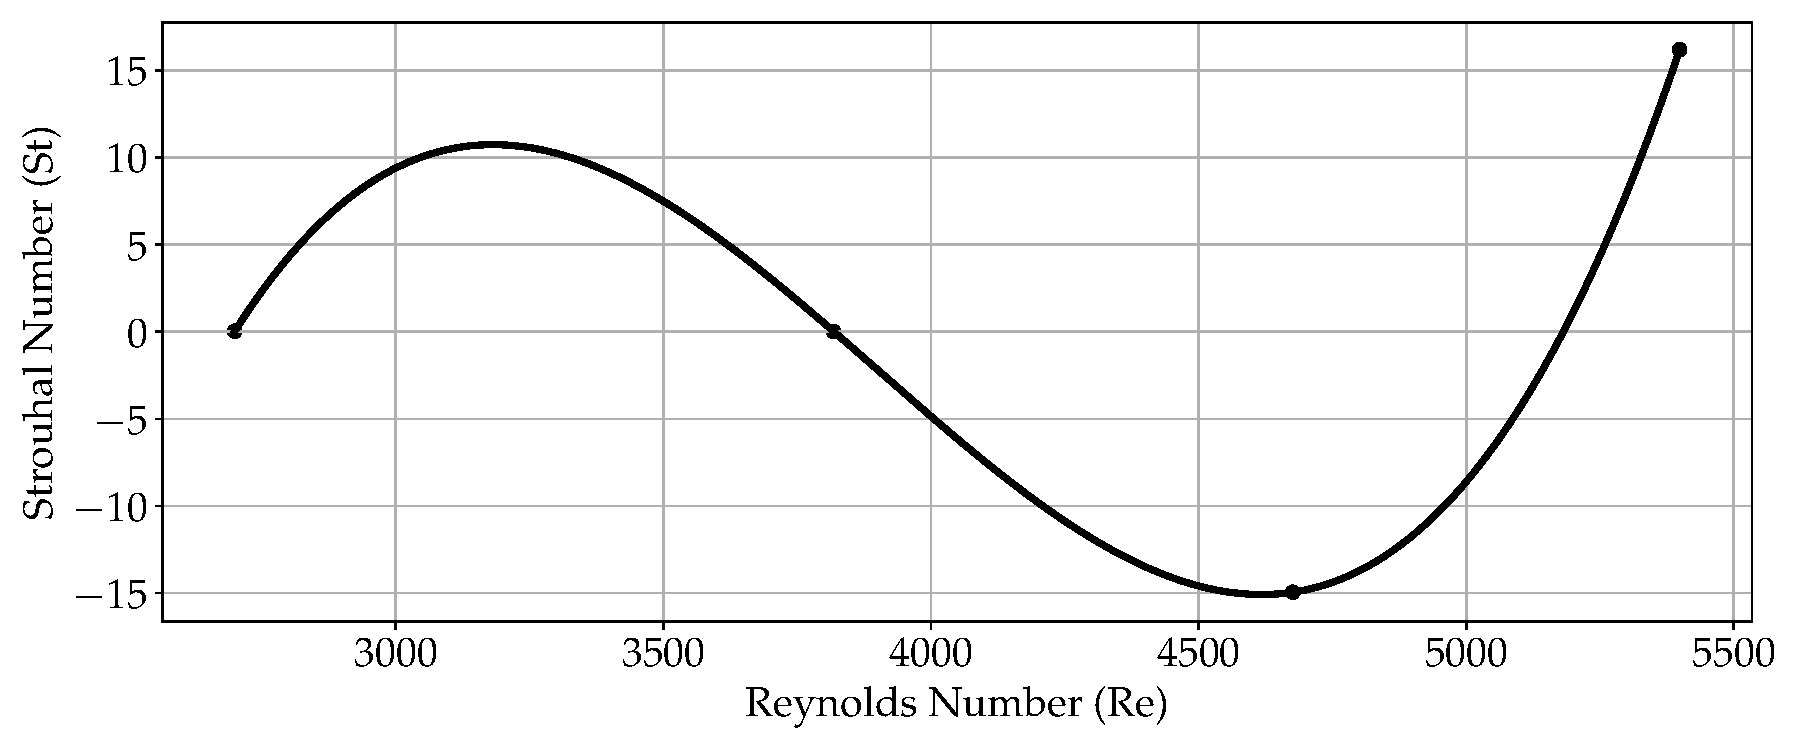
\includegraphics[width=\linewidth]{gfx/Re_vs_St_x_4D_y_0-5_D.pdf}
    \caption{Variation of Strouhal number ($St$) with Reynolds number ($Re$) for flow past a cylinder at a distance of \enquote{$4~D$} and a height of \enquote{$0.5~D$} from the center of the cylinder.}
    \label{fig:st_vs_re_x_4D_y_0-5_D}
\end{figure}

\section{Chapter summary}
In this chapter, the vortex shedding analysis for a flow with differential pressures of $1~Pa$, $2~Pa$, $3~Pa$ and $4~Pa$ is discussed. For this analysis, a hot wire anemometer calibrated using a pitot static tube is used. The vortex shedding behavior is studied at various locations in the test section of the wind tunnel. The solid cylinder with diameter $D = 0.033~m$ is placed at a distance of $0.2~m$ from the left end of the test section. The hot wire anemometer is placed at a distance of $D$, $2~D$ and $4~D$ from the center of the cylinder and at a height of $0.5~D$ from each location. The voltage variation of the sensor is measured and its corresponding velocity variation is calculated using the calibration equation (Eq.~(\ref{eq:calib_eqn_hwa})) in temporal domain. Then it is converted to the frequency domain using the forward Fourier transform equation (Eq.~(\ref{eq:forward fourier})). The peak frequency of the vortex is calculated at each point and the corresponding Strouhal number (Eq.~(\ref{strouhal number})) is calculated. The variation of Strouhal number is plotted with Reynolds number at all six locations. The Strouhal number is found to vary between 0 and 0.2 in some locations, and it is deviating very largely at other locations. This is due to the flow transition from laminar region to turbulence.